\documentclass[handout]{beamer}
\usepackage[latin1]{inputenc}
\usepackage{bm, array, graphicx, hyperref, amsmath, setspace, geometry, wrapfig}
\usepackage{hanging}
%\usepackage{datetime}
\usetheme{Warsaw}
\title{Introduction to Nuclear Magnetic Resonance Spectroscopy}
\author{Dr Alexey Potapov}
\institute{University of Nottingham, School of Physics and Astronomy}
%\date{Jule 13, 2017}
%\newdate{date}{06}{09}{2012}
%\date{\displaydate{date}}
\date{\today}

\setbeamertemplate{headline}{}
\setbeamertemplate{footline}{}
\setbeamertemplate{caption}{Fig.\insertcaptionnumber: \insertcaption \par}
\setbeamerfont{caption}{size=\scriptsize }
\setbeamercovered{invisible}
\setbeamercovered{%
	again covered={\opaqueness<1->{50}}}
%\newenvironment{slide}[1]
%{\begin{frame}[environment=slide]
%		\frametitle{\insertsection-#1}}
%	{\end{frame}}
\newcolumntype{C}[1]{>{\centering\arraybackslash}m{#1}}
\setbeamertemplate{footnote}{%
	\hangpara{2em}{1}%
	\makebox[2em][1]{\insertfootnotemark}\footnotesize\insertfootnotetext\par%
}

%%%%%%%%define the begin section slide
\AtBeginSection[]{
	\begin{frame}
		\vfill
		\centering
		\begin{beamercolorbox}[sep=8pt,center,shadow=true,rounded=true]{title}
			\usebeamerfont{title}\insertsectionhead\par%
		\end{beamercolorbox}
		\vfill
       \tableofcontents[
       sectionstyle=hide/hide,
       subsectionstyle=show/show/hide]
	\end{frame}
}
%%%%%%%%%%



\begin{document}
	
	\begin{frame}
		\titlepage
	\end{frame}
	
	\section{Introduction. Magnetic moment in magnetic field.}
	\subsection{Introduction to Magnetic Resonance}	
	\begin{frame}{\thesection.\thesubsection. \insertsubsection}

		
		\begin{itemize}
		\item Magnetic resonance (MR) is a phenomenon of resonant energy absorption by a system of nuclei (and electrons). 
		\item Nuclear magnetic resonance (NMR) results from the intrinsic magnetic moment of the
		nuclei of some atoms. Magnetic moments of electrons are exploited in electron spin resonance (ESR).
		\item Magnetic resonance (MR) generally involves placing a sample in a strong magnetic
		field (to generate polarisation at a fixed resonant frequency) and detecting signals
		produced following application of pulsed radio-frequency electromagnetic fields (RF
		pulses).
		\item MR is a very powerful method for studying the structure of materials: used in physics, chemistry, biology, medicine etc.

		\end{itemize}
	\end{frame}
	
	\subsection{Applications of NMR}
	\begin{frame}{\thesection.\thesubsection. \insertsubsection}
	 \begin{itemize}
	 	\item NMR spectroscopy is used for chemical analysis and for molecular structure determination	  	
	 \end{itemize}
		
		\begin{figure}[ht]
			\begin{minipage}[t]{0.45\linewidth}
				\centering
				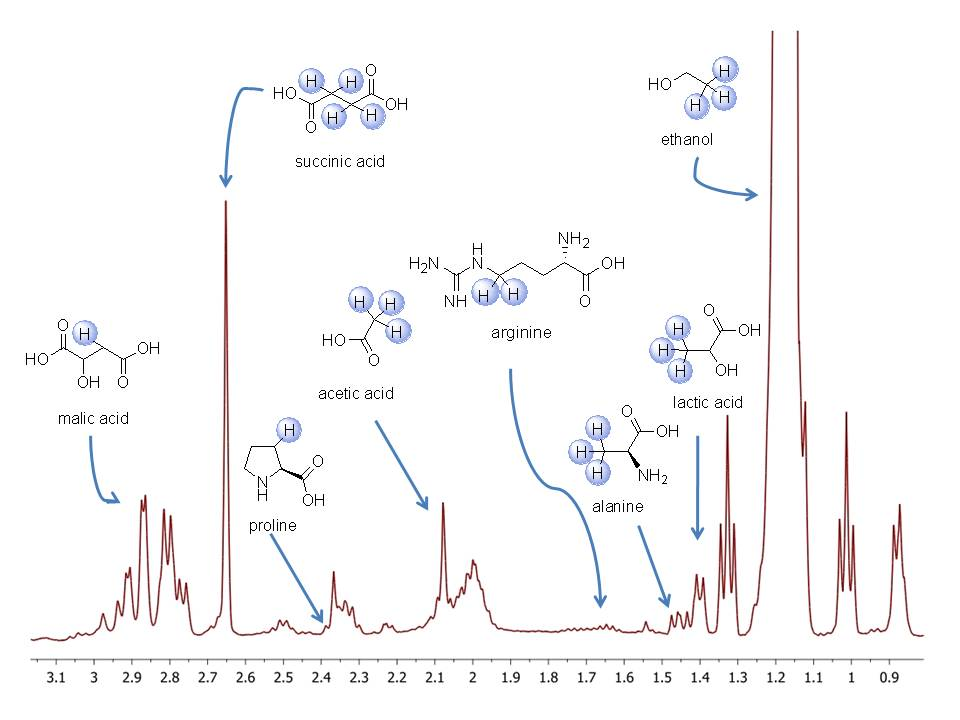
\includegraphics[width=\textwidth]{wine_spectrum.jpg}
				\caption{\textsuperscript{1}H NMR spectrum of a sample of Spanish wine (\url{http://www.unirioja.es/gsoe/NMR.htm})}
				\label{fig1}
			\end{minipage}
			\hspace{0.3cm}
			\begin{minipage}[t]{0.45\linewidth}
				\centering
				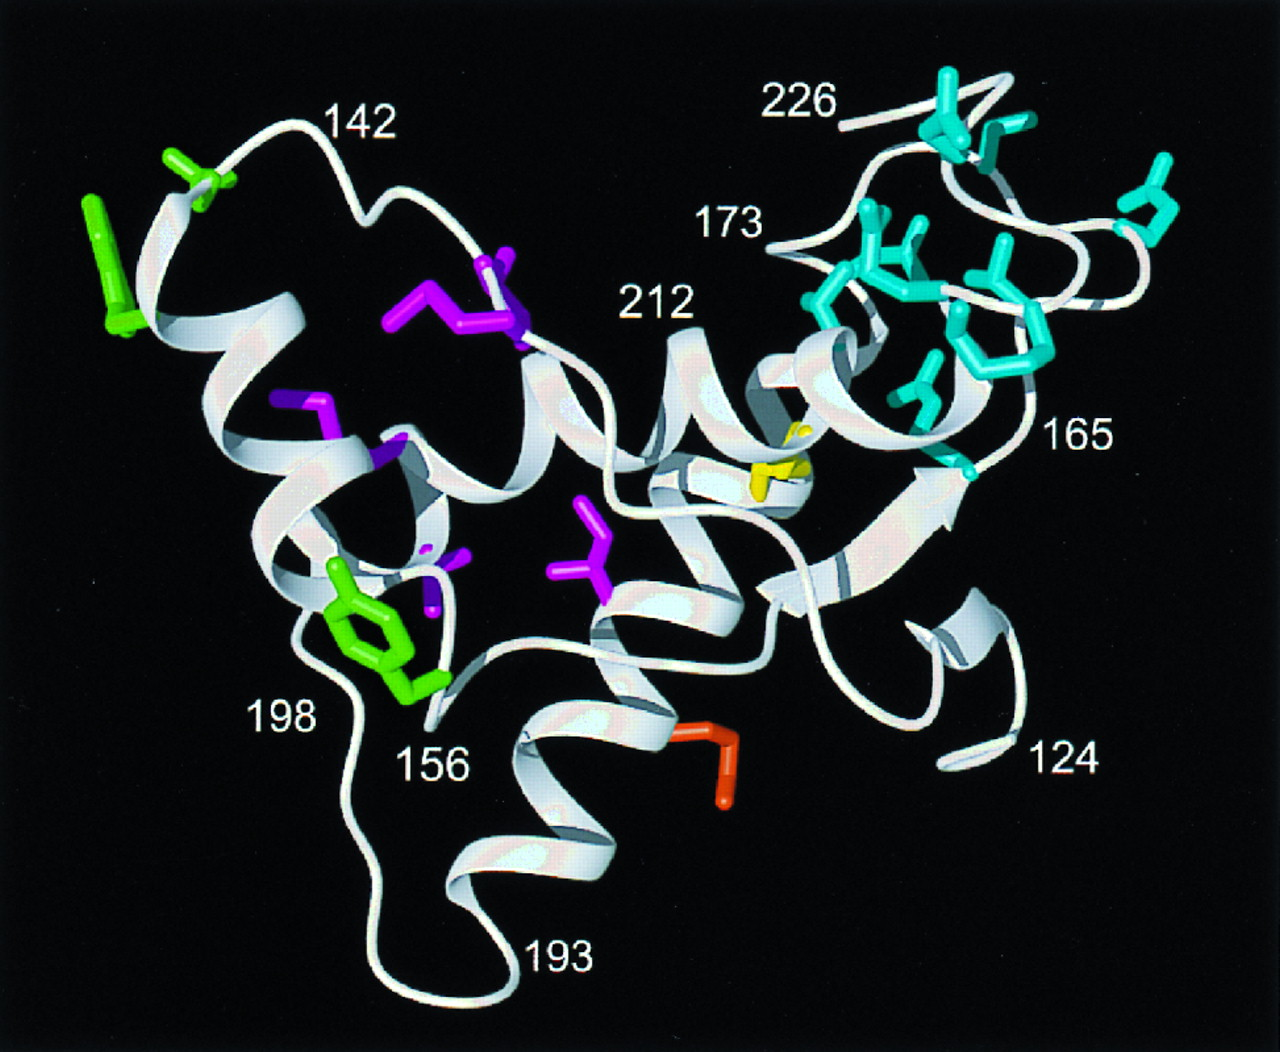
\includegraphics[width=\textwidth]{prion.jpg}
				\caption{NMR-derived structure of a prion  \url{http://www.pnas.org/content/94/14/7281.full}}
				\label{fig3}
			\end{minipage}					
		\end{figure}
	\end{frame}
	
	
	\begin{frame}{\thesection.\thesubsection. \insertsubsection}
		\begin{itemize}
			\item NMR relaxometry can be used to monitor molecular environment
		\end{itemize}

		\begin{figure}[ht]
					
						
			\begin{minipage}[t]{0.15\textwidth}
				\centering
				(a)
				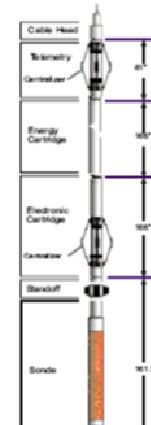
\includegraphics[width=\textwidth]{well_logging1.jpg}
			\end{minipage}
			\hspace{0.1cm}
			\begin{minipage}[t]{0.15\textwidth}
				\centering
				(b)
				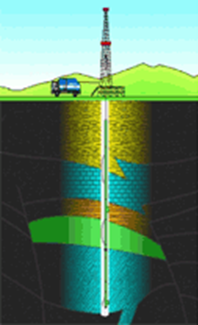
\includegraphics[width=\textwidth]{well_logging2.png}
				\label{fig7}
			\end{minipage}			
			\hspace{0.1cm}				
			\begin{minipage}[t]{0.15\textwidth}
				\centering
				(c)
				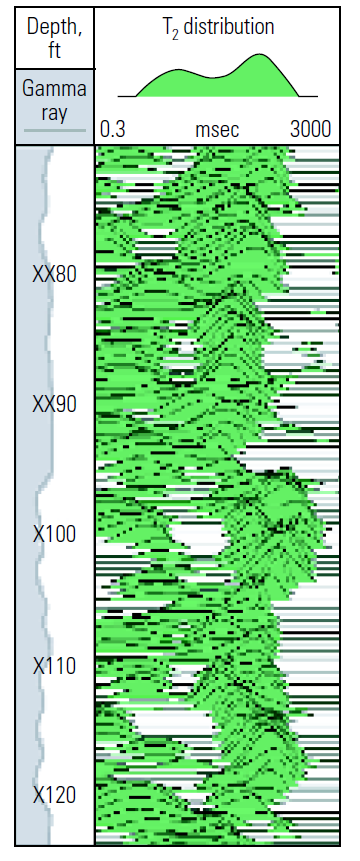
\includegraphics[width=\textwidth]{well_logging3.png}	
				\label{fig5}
			\end{minipage}		
			\hspace{0.1cm}
			\caption{ (a) NMR-logging probe, (b) Schematic positioning of the probe in a well, (c) T\textsubscript{2}-relaxation profile along the bore. Sources: 1) Allenet al. Oilfield review, Autumn 2000; 2) Coates, Xiao NMR Logging Principles and Applications, Hulliburton}		
		\end{figure}			
	\end{frame}
	
\begin{frame}{\thesection.\thesubsection. \insertsubsection}
	\begin{itemize}
		\item NMR forms the basis for magnetic resonance imaging (MRI)
	\end{itemize}
	
	\begin{figure}[ht]
			\centering
			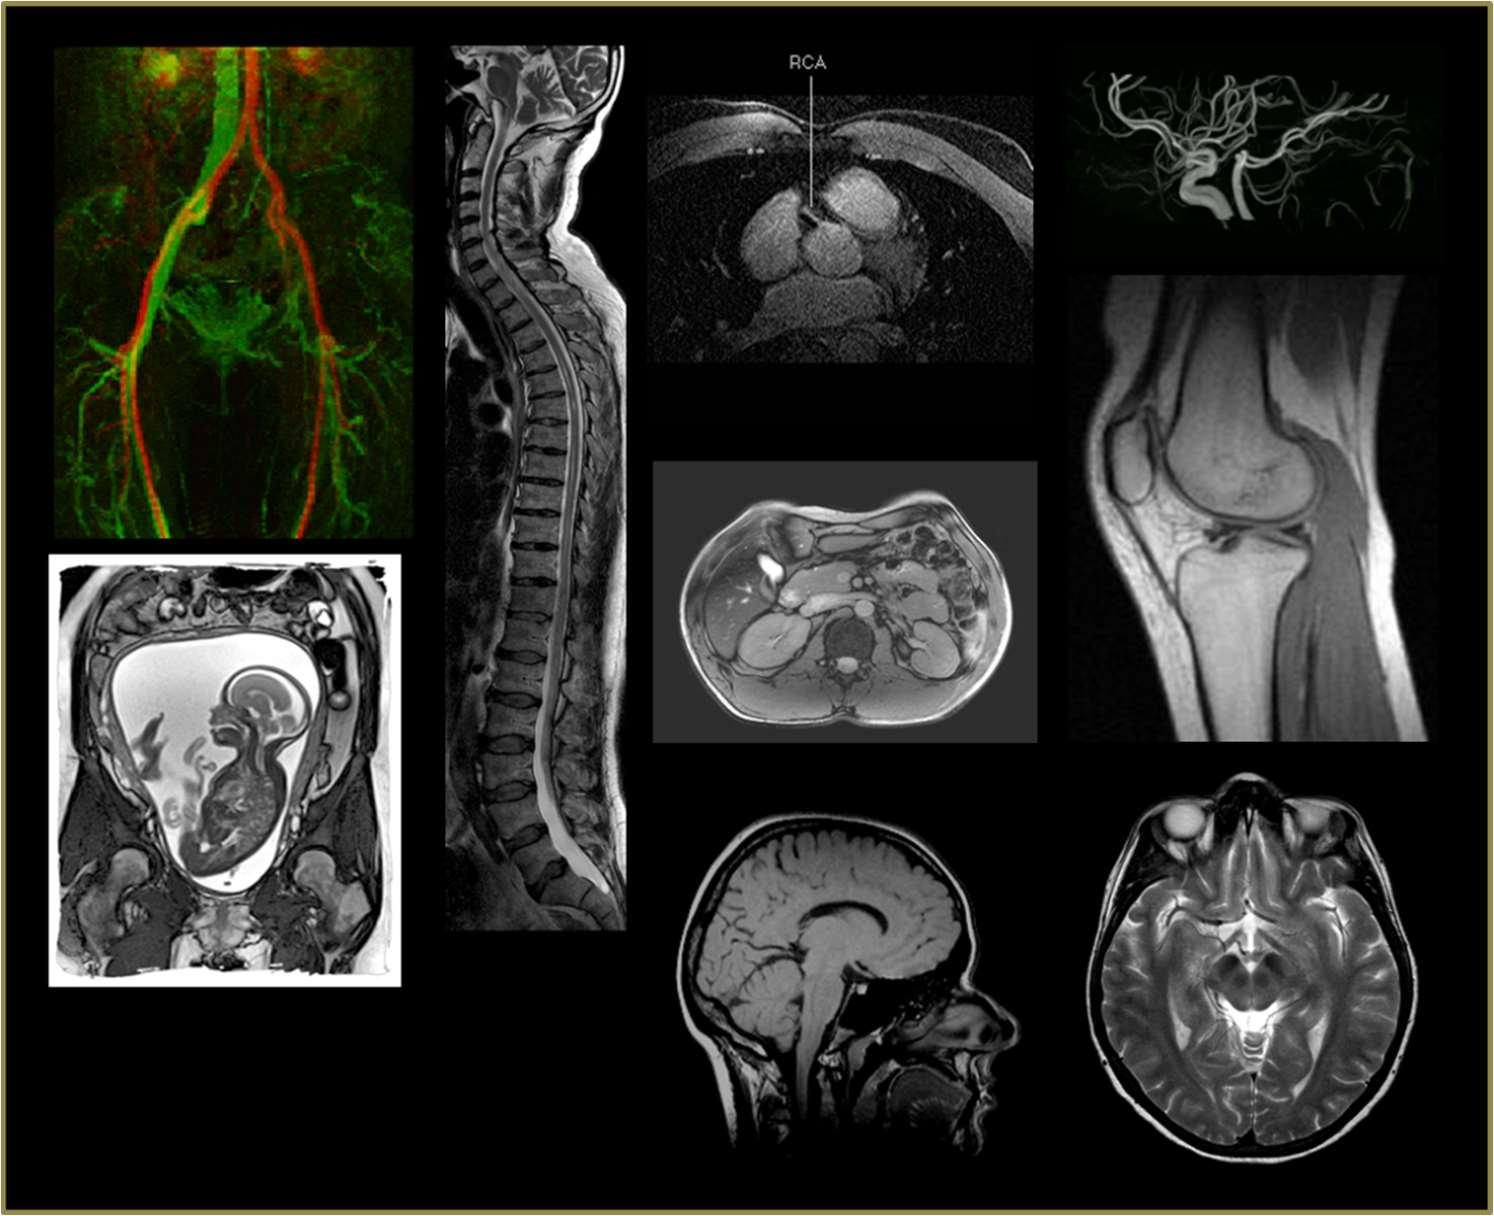
\includegraphics[width=0.7\textwidth]{mri.jpeg}
		\caption{  Example magnetic resonance images of blood vessel (in legs), fetus in utero, spine, heart, abdomen, head, blood vessels (in brain), knee, brain (courtesy of Prof. Richard Bowtell)}		
	\end{figure}			
\end{frame}


\subsection{Magnetic moments in magnetic field.}

\begin{frame}{\thesection.\thesubsection. \insertsubsection}
	
	\begin{itemize}[<+>]
		\item Consider charges moving in a limited volume. The position of a charge $\bm{e_n}$ will be given by a vector $\bm{r_n}$ and its velocity by $\bm{v_n}$. The overall magnetic moment of such a system is defined as:
			
			\begin{equation}
			\bm{M} = \frac{1}{2} \sum_{n} e_n\bm{r_n} \times \bm{v_n}
			\end{equation}
		\item 	If all the charges and masses are the same, then $\bm{M}$ can be rewritten as:	
			\begin{equation} \label{eq:1}
			\bm{M} = \frac{e}{2m} \sum_{n} m\bm{r_n} \times \bm{v_n} = \gamma \bm{L},
			\end{equation}
			where
			\begin{equation}
			\bm{L} = \sum_{n} \bm{p_n} \times \bm{r_n}
			\end{equation}
			is the mechanical angular momentum.
		\item 
			\alert{Gyromagnetic ratio} (or magnetogyric): 
			\begin{equation}
			\gamma = \dfrac{e}{2m}
			\end{equation}
			
	
	\end{itemize}
	


\end{frame}

\begin{frame}{\thesection.\thesubsection. \insertsubsection}
	\begin{itemize}[<+>]
		\item When a magnetic moment $\bm{M}$ is placed into an external uniform permanent magnetic field $\bm{B}$, its energy is given by:
			
			\begin{equation} \label{eq:classic_energy}
			E = -\bm{M} \cdot \bm{B}
			\end{equation} 
		\item  The torque acting on the system:
			\begin{equation}
			\frac{d\bm{L}}{dt} = \bm{M} \times \bm{B}
			\end{equation}
			  
		 \item  	Now using equation \ref{eq:1} we can obtain the equation describing the motion of vector $\bm{M}$:
			
			\begin{equation} \label{eq:precession_compact}
			\frac{d\bm{M}}{dt} = \gamma \bm{M} \times \bm{B}
			\end{equation}
			
	\end{itemize}
\end{frame}
\begin{frame}{\thesection.\thesubsection. \insertsubsection}
	\begin{itemize}[<+>]
		\item 
		    In a uniform magnetic field directed along $z$-axis $\bm{B} = (0, 0, B_0)$, the equation for individual components of $\bm{M}$ follow the equations:
		    
		    \begin{minipage}[b][4cm]{0.4\textwidth}
		    	\centering
		    	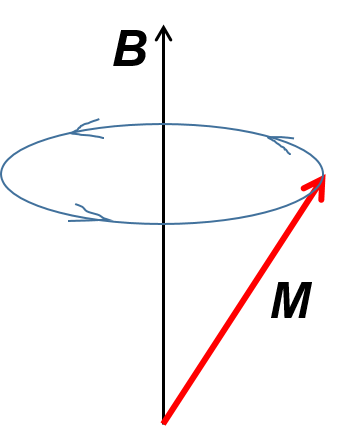
\includegraphics[width=0.7\textwidth]{precession.png}
		    \end{minipage}
		    \hspace{0.1cm}		    
		    \begin{minipage}[b][4cm]{0.4\textwidth}
		        \centering
		    	 \begin{equation} \label{precession}
		    	 \setlength{\jot}{5pt}
		    	 \begin{aligned}
		    	 \dfrac{dM_x}{dt} & =  \omega_L M_y \\
		    	 \dfrac{dM_y}{dt} & =  -\omega_L M_x \\
		    	 \dfrac{dM_z}{dt} & =  0,
		    	 \end{aligned}
		    	 \end{equation}
		    	 where $\omega_L = \gamma B_0$ - \alert{Larmor frequency}.
		    \end{minipage}
		    
		    
		\item
			A solution to this system of differential equations with initial values of $M_x(0), M_y(0), M_z(0)$ has the following form:
						
			\begin{equation} 
			\begin{array}{lcl}
			M_x(t) &=& M_x(0) \cos(\omega_L t) + M_y(0) \sin (\omega_L t) \\
			M_y(t) &=& -M_y(0) \sin(\omega_L t) + M_y(0) \cos (\omega_L t) \\
			M_z(t) &=& M_z(0) 
			\end{array}
			\end{equation}
		
		
	\end{itemize}
		
\end{frame}

\subsection{Orbital angular momentum operator}
\begin{frame}{\thesection.\thesubsection. \insertsubsection}
	
	\begin{itemize}[<+>]
		\item     In quantum mechanics physical quantity $A$ ise represented by an operator $\hat{A}$. The mechanical angular momentum is replaced by its corresponding operator:
		\begin{equation}
		\bm{L} = \sum_{n} \bm{p_n} \times \bm{r_n}  \longleftrightarrow \bm{\hat{L}} = \dfrac{1}{\hbar} \sum_{n} \bm{\hat{r}_n} \times \bm{\hat{p}_n} =   -i \sum_{n} \bm{\hat{r}_n} \times \bm{\nabla_n}
		\end{equation}
		\item Angular momentum operator properties. Commutation:
		\begin{equation}\label{eq:Lz_commutation}
		  [\hat{L}_y,\hat{L}_z] = i\hat{L}_x, [\hat{L}_z,\hat{L}_x] = i\hat{L}_y, [\hat{L}_x,\hat{L}_y] = i\hat{L}_z
    	\end{equation}
		\item Angular momentum squared, and its commutation properties:
        \begin{align}
          &\hat{L}^2 = \hat{L}_x^2 + \hat{L}_y^2 + \hat{L}_z^2 \\
          &[\hat{L}^2, \hat{L}_x]=[\hat{L}^2, \hat{L}_y]=[\hat{L}^2, \hat{L}_z]= 0       
        \end{align}        
	\end{itemize}

\end{frame}

\begin{frame}{\thesection.\thesubsection. \insertsubsection}
	\begin{itemize}[<+>]
		\item Eigenfunctions of both $\hat{L}^2$ and $\hat{L}_z$ operators can be characterized by integer quantum numbers $l$  and $m$ respectively. These eigen functions will be denoted as $\vert lm \rangle$. Their eigenvalues are:
		\begin{align}
		\hat{L}_z \vert lm \rangle &= m \vert lm \rangle \\
		\hat{L}^2 \vert lm \rangle &= l(l+1) \vert lm \rangle
		\end{align}
		\item Another useful operator are raising and lowering operators:
		\begin{align}
		  &\hat{L}_{+} = \hat{L}_x + i\hat{L}_y, \hat{L}_{-} = \hat{L}_x - i\hat{L}_y\\
		  &\langle lm \vert \hat{L}_{+} \vert l (m-1) \rangle = \langle l(m-1) \vert \hat{L}_{-} \vert lm \rangle = \sqrt{(l+m)(l-m+1)} \label{eq:L+}
		\end{align}
	\end{itemize}
	
\end{frame}

\begin{frame}
		\begin{block}{Problem}
			Calculate $[\hat{L}_{+}, \hat{L}_x ] = ?$ , $[\hat{L}_{+}, \hat{L}_{-} ] = ?$ 
		\end{block}
		\begin{equation*}
		[\hat{L}_y,\hat{L}_z] = i\hat{L}_x, [\hat{L}_z,\hat{L}_x] = i\hat{L}_y, [\hat{L}_x,\hat{L}_y] = i\hat{L}_z
		\end{equation*}
		\begin{align*}
		&\hat{L}^2 = \hat{L}_x^2 + \hat{L}_y^2 + \hat{L}_z^2 \\
		&[\hat{L}^2, \hat{L}_x]=[\hat{L}^2, \hat{L}_y]=[\hat{L}^2, \hat{L}_z]= 0    \\   
	    &\hat{L}_{+} = \hat{L}_x + i\hat{L}_y, \hat{L}_{-} = \hat{L}_x - i\hat{L}_y
		\end{align*}        


\end{frame}




\begin{frame}{\thesection.\thesubsection. \insertsubsection}
	\begin{itemize}[<+>]
		\item
			Classical magnetic moment will have its own quantum analogue, the operator of angular momentum:
			\begin{equation}\label{eq:orbital_angular_momentum}
			\bm{M} = \gamma \bm{L}  \longleftrightarrow \bm{\hat{\mu}} = \gamma \hbar \bm{\hat{L}}
			\end{equation} 
		\item Given the electron charge $e= 1.6 \cdot 10^{-19}$C, and mass $m = 9.1 \cdot 10^{-31}$kg   \alert{Bohr magneton}:
		\begin{equation}
			\beta_e = \gamma \hbar = \dfrac{e\hbar}{2m} \approx 9.27 \cdot 10^{-24}  \text{J$\cdot$T}^{-1}
		\end{equation}
		\item Similarly a \alert{nuclear magneton} could be calculated for a proton (\textsuperscript{1}H nucleus):
		\begin{equation}
		\beta = \gamma_N \hbar = \dfrac{e\hbar}{2m_p} \approx 5.05 \cdot 10^{-27}  \text{J$\cdot$T}^{-1}
		\end{equation}
		
	\end{itemize}

\end{frame}

\subsection{Spin angular momentum operator}
\begin{frame}{\thesection.\thesubsection. \insertsubsection}
	However, real nuclei and electrons have spins (intrinsic magnetic moment). Their z-axis projection $m$ takes integer and half-integer values: $m=\dfrac{1}{2}, 1, \dfrac{3}{2}, 2$ etc. Similar to the equation for the orbital angular momentum Eq.\ref{eq:orbital_angular_momentum}. For nuclei spins we get its magnetic moment as:
	\begin{equation}
		\bm{\hat{\mu}_N} = \gamma_N \hbar \bm{\hat{I}},
	\end{equation}
	where $ \bm{\hat{I}}$ stands for the nuclear spin operator. All the properties of angular momentum operators listed in Eqs.\ref{eq:Lz_commutation}-\ref*{eq:L+} will be true for $ \bm{\hat{I}}$.
\end{frame}

\begin{frame}{\thesection.\thesubsection. \insertsubsection}
	\begin{itemize}[<+>]
		\item 	Many nuclei in the periodic table are magnetic, i.e. have spin $I \neq 0$. Their magnetic moments could be measured in units of $\beta_N$:
		\begin{equation}
		\bm{\hat{\mu}_N} = \gamma_N \hbar \bm{\hat{I}} = g_N \beta_N \bm{\hat{I}},
		\end{equation}
		where $g_N$ - dimensionless g-factor.
		\item
% TABLE OF MAGNETIC PROPERTIES
\begin{table}[ht]
	\centering
	\begin{tabular}{  C{1.0cm}  C{2.0cm}  C{1.0cm}  C{2.cm}  C{3cm}}
		\hline\hline
		Nucleus & Natural abundance \% & Nuclear spin (I) & $g_N$, g-factor & $\gamma_N$, Gyromagnetic ratio ($10^7$ rad/T*s) \\
		\hline
		\textsuperscript{1}H & 99.98 & $\frac{1}{2}$ & 5.585 & 26.7519 \\
		\textsuperscript{2}H & 1.5*10\textsuperscript{-2} & 1 & 0.857 & 4.1066 \\
		\textsuperscript{13}C & 1.108 & $\frac{1}{2}$ & 1.405 & 6.7283 \\
		\textsuperscript{14}N & 99.635 & 1 & 0.403 & 1.9338 \\
		\textsuperscript{15}N & 0.365 &  $\frac{1}{2}$ & -0.567 & -2.712 \\
		\hline
	\end{tabular}
	%\caption{Magnetic properties of some common nuclei. More can be found at \url{http://www.bruker-nmr.de/guide/eNMR/chem/NMRnuclei.htm} }
	\label{tab:mag_properties}		
\end{table}
%%%%% END OF TABLE	
	\item
    Electron magnetic moments can be measured in units of Bohr magnetons: $\bm{\hat{\mu}_S} = -\gamma_e \hbar \bm{\hat{S}} = -g_e \beta_e \bm{\hat{S}}$, and for a free electron spin $g_e \approx 2.0023$.		
	\end{itemize}
\end{frame}


\begin{frame}{Summary of Lecture 1}
	\begin{itemize}
		\item Applications of NMR: chemistry, biology, medicine, industry ...
		\item Magnetic moment in magnetic field: Classical description 
		\item Recap of angular momentum operator properties: commutation properties.
		\item Nuclei have their own nuclear magnetic moment. Described using spin angular momentum operator.
	\end{itemize}
	\textbf{Suggested reading: } Harris: 1.1, 1.2, 1.3, 1.4, 1.6, 2.4
\end{frame}



\subsection{Spin in a magnetic field}
\begin{frame}{\thesection.\thesubsection. \insertsubsection}
		\begin{itemize}[<+>]
		\item Let's quantum mechanically describe the system of spins in the magnetic field. Eq. \ref{eq:classic_energy} can be rewritten in a form of Hamiltonian:
		\begin{equation}
			E = -\bm{M} \cdot \bm{B}  \longleftrightarrow \mathcal{H}= - \bm{\hat{\mu}_N} \cdot \bm{B} 
		\end{equation}
		\item when the magnetic field is directed along z-axis $\bm{B}= (0,0,B_0)$:
		\begin{equation}
		\mathcal{H}= - \bm{\hat{\mu}_N} \cdot \bm{B} = -\gamma_N \hbar B_0 \hat{I}_z
		\end{equation}
		\item For spin $I=\dfrac{1}{2}$ such Hamiltonian produces a two-level system. Its energy levels corresponding to eigenfunctions $\vert \alpha \rangle$ and $\vert \beta \rangle$:
		\begin{figure}
		    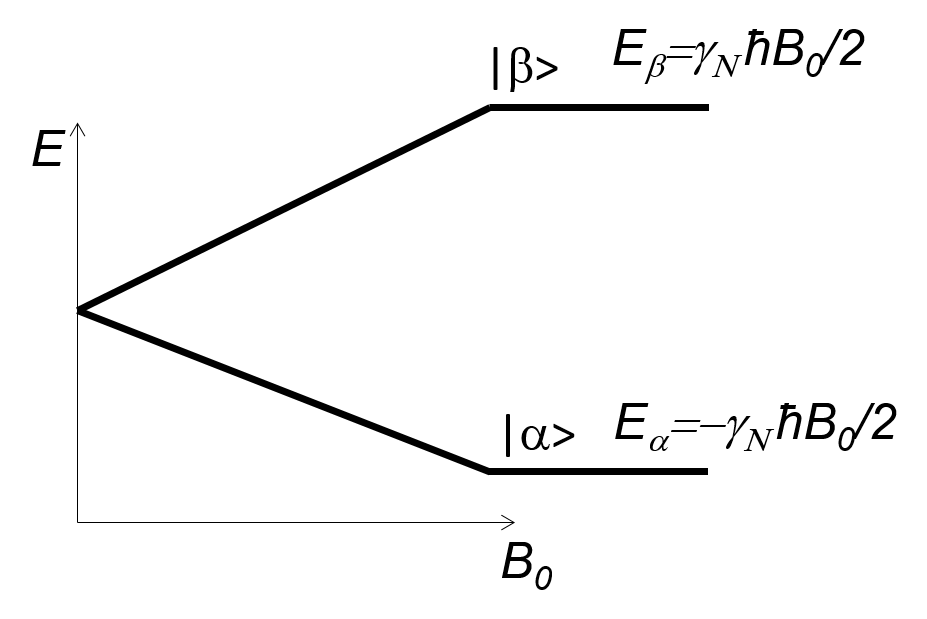
\includegraphics[width=0.5\textwidth]{two-level_system.png}
		\end{figure}
		
	\end{itemize}
\end{frame}

\begin{frame}{\thesection.\thesubsection. \insertsubsection}
	\begin{itemize}[<+>]
		\item The transition between the two states requires an energy quantum\footnote{More can be found in Bruker Almanac at https://lsa.umich.edu/content/dam/chem-assets/chem-docs/BrukerAlmanac2011.pdf}:
		\begin{equation}
			h \nu_L = \gamma \hbar B_0, \omega_L = \gamma B_0, \nu_L = \dfrac{\gamma B_0}{2 \pi}
		\end{equation}
		$\omega_L$ and $\nu_L$ is the Larmor frequency (anglular and cyclic respectively)
		\item
		
% TABLE OF MAGNETIC PROPERTIES
\begin{table}[ht]
	\centering
	\begin{tabular}{  C{1.0cm}  C{2.5cm}  C{1.0cm}  C{2.0cm}  C{2.0cm}}
		\hline\hline
		Nucleus & Natural abundance \% & Nuclear spin (I) & Larmor frequency at 11.744T, MHz & $\gamma_N$, Gyromagnetic ratio ($10^7$ rad/T*s) \\
		\hline
		\textsuperscript{1}H & 99.98 & $\frac{1}{2}$ & 500 & 26.7519 \\
		\textsuperscript{2}H & 1.5*10\textsuperscript{-2} & 1 & 76.753 & 4.1066 \\
		\textsuperscript{13}C & 1.108 & $\frac{1}{2}$ & 125.721 & 6.7283 \\
		\textsuperscript{14}N & 99.635 & 1 & 36.118 & 1.9338 \\
		\textsuperscript{15}N & 0.365 &  $\frac{1}{2}$ & 50.664 & -2.712 \\
		\hline
	\end{tabular}
\end{table}
%%%%% END OF TABLE
		
	\end{itemize}
\end{frame}

\subsection{Equilibrium magnetization}
\begin{frame}{\thesection.\thesubsection. \insertsubsection}
  NMR measurements are generally made on bulk samples which contain very large numbers of nuclear spins (e.g. 1 cm$^3$ contains $N \approx 6.7 \cdot 10^{22}$ \textsuperscript{1}H atoms)
  The measured signals therefore result from the collective effect of a large number of magnetic moments that can be described using a bulk magnetization.
  At thermal equilibrium, the numbers of nuclei in the $\vert \alpha \rangle$ state $N_{\alpha}$ and  $\vert \beta \rangle$ state $N_{\beta}$ follow Boltzmann distribution:
  \begin{equation}
    \dfrac{N_{\alpha}}{N_{\beta}} = e^{-\dfrac{\gamma B_0}{kT}} \approx (1 - \dfrac{\gamma B_0}{kT}),
  \end{equation} 
  when $\gamma B_0 \ll kT$. Overall magnetization then can be calculated as:
  \begin{equation}
    M_z = N_{\alpha}(-\dfrac{1}{2}\gamma \hbar) + N_{\beta}(\dfrac{1}{2}\gamma \hbar) = N \dfrac{\gamma^2 \hbar^2 B_0}{4kT} 
  \end{equation}
\end{frame}

\begin{frame}
	\begin{block}{Problem}
		\begin{itemize}
			\item What is the value of $\dfrac{\gamma_N \hbar B_0}{kT}$ for proton nuclei (\textsuperscript{1}H) at $9.4$ T magnetic field at 300 K?
			\item What is the value of $\dfrac{\gamma_e \hbar B_0}{kT}$ electron (\textsuperscript{1}H) at $9.4$ T magnetic field at 4 K?
		\end {itemize}      
	\end{block}
	{\tiny
	\begin{align*}
	&\text{Electron charge } e = 1.602 \cdot 10^{-19} \text{C}\\
	&\text{Electron mass } m_e = 9.109 \cdot 10^{-31} \text{kg} \\
	&\text{Proton mass}  m_p =  1.673 \cdot 10^{-27} \text{kg}  \\
	&\text{Plank constant}  \hbar =  1.054 \cdot 10^{-34} \dfrac{\text{J} \cdot \text{s}}{rad}  \\
	&\text{Proton g-factor}  g_p =  5.585 \\
	&\text{Electron g-factor}  g_e =  2.0023 \\
	&\text{Nuclear magneton}  \beta_N =  5.05 \cdot 10^{-27}  \text{J}\cdot \text{T}^{-1} \\
	&\text{Bohr magneton}  \beta_e =  9.27 \cdot 10^{-24}  \text{J}\cdot \text{T}^{-1} \\
	&\text{Proton gyromagnetic ratio}  \gamma_N =  26.7519 \cdot 10^{7} \dfrac{\text{rad}}{T \cdot s}\\
	&\text{Electron gyromagnetic ratio}  \gamma_e =  1.76 \cdot 10^{11} \dfrac{\text{rad}}{T \cdot s}\\
	&\text{Boltzmann constant}  k =  1.38 \cdot 10^{-23} {\text{J}} \cdot \text{K}^{-1}\\
	&\text{Avogadro's constant}  N_A =  6.023 \cdot 10^{23} \text{mol}^{-1}
	\end{align*}
    }%
\end{frame}
\subsection{Resonant energy absoption.}
%%%%%RESONANT ABSORBTION SECTION

\begin{frame}{\thesection.\thesubsection. \insertsubsection}

	\begin{itemize}[<+>]

		\item[]
		{\small
		Let's apply oscillating magnetic field to our system. A spin system Hamiltonian becomes time-dependent and for an oscillation along the $x$-axis we obtain:
		\begin{equation} \label{eq:oscillating_field}
		\begin{array}{lcl}
		\mathcal{H}(t) &=& -\bm{\hat{\mu}} \bm{(B_0+B(t))}=  \\
		&=& -\gamma \hbar \hat{I_z} (B_0 + B_1(t)) =\\
		&=&-\gamma \hbar \hat{I_z} B_0  -\gamma \hbar \hat{I_x} B_1 \cos(\omega t),
		\end{array}
		\end{equation}
		where $H_1$ and $\omega$ are the amplitude and the frequency of the oscillating magnetic field.
	}%
		\item[]
				{\small
		According to perturbation theory the transition probability between the initial state $\vert a \rangle$ and the final state $\vert b \rangle$ with a time dependent Hamiltonian $ \hat{V} (t) = 2 \hat{F} \cos (\omega t ) $ is (Fermi's golden rule):
		\begin{equation} \label{eq:probability}
		P_{ab} = \frac{2 \pi}{\hbar} \vert \langle a \vert \hat{F} \vert \rangle b \vert ^2 \delta(E_{ab}-\hbar \omega),
		\end{equation}
		where $E_{ab} = E_a - E_b$ is an energy difference between the energies of levels $a$ and $b$. \\		
		\textbf{Note!} The matrix element $\vert \langle a \vert \hat{F} \vert \rangle b \vert$ represents the selection rules for various levels, if it equals to zero, the transition in 
		forbidden, otherwise - allowed.		    
	}%
	\end{itemize}

\end{frame}	
\subsection{Populations dynamics in two-level system.}
\begin{frame}{\thesection.\thesubsection. \insertsubsection}
	\begin{itemize}[]
		\item 
		For a two level system described before, the matrix element $\langle \alpha \vert \hat{I_x} \vert \beta \rangle = \frac{1}{2}$. The transition probability then becomes:
		\begin{equation}\label{eq:two level transition probability}
		P_{\alpha \beta} = \frac{\pi}{2\hbar} (\gamma H_1)^2 \delta(E_{\alpha \beta}-\hbar \omega),
		\end{equation}
		\begin{minipage}{1.0\textwidth}
			\centering
			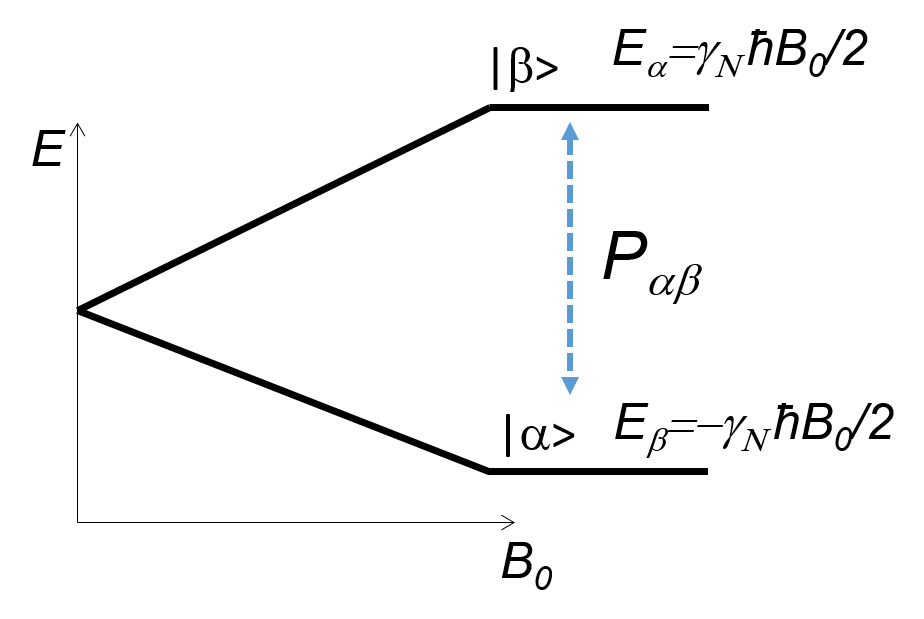
\includegraphics[width=0.5\textwidth]{two-level_excite.png}
		\end{minipage}
		\item
		\textbf{The effect of resonant absorption (and emission) of electromagnetic irradiation at the frequency matching the energy difference in a nuclear system is called Nuclear Magnetic Resonance (NMR).} 		    
		
		
	\end{itemize}
	
\end{frame}	

\begin{frame}{\thesection.\thesubsection. \insertsubsection}
	\begin{itemize}[<+>]
	\item In a two-level system the transition will take place due to the action of external irradiation, but also due to interaction with the environment.
	\begin{minipage}{1.0\textwidth}
		\centering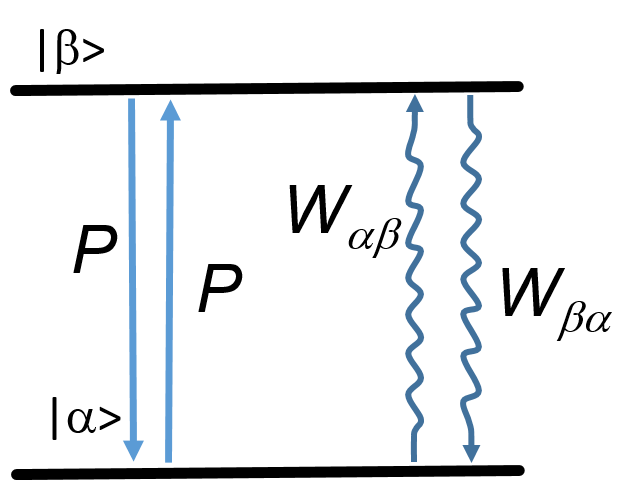
\includegraphics[width=0.3\textwidth]{two_level_population.png}
	\end{minipage}
	$P$ - the rate of transitions driven by external field, $W_{\alpha \beta}, W_{\beta \alpha}$ - rates of spontaneous spin flips due to interaction with environment.
	\item
	In thermal equilibrium:
	\begin{align}
		&N_{\alpha}^0 W_{\alpha \beta} = N_{\beta}^0 W_{\beta \alpha}, \text{i.e.} \\
		&\dfrac{ W_{\beta   \alpha }}{ W_{\alpha  \beta  }} = exp^{-\dfrac{\gamma \hbar B_0}{kT}} \approx 1-\dfrac{\gamma \beta B_0}{kT}
	\end{align}
	\end{itemize}
\end{frame}

\begin{frame}{\thesection.\thesubsection. \insertsubsection}
	\begin{itemize}[<+>]
		\item Equation for populations of levels:
		\begin{equation}
		\begin{array}{lcl}
		\dfrac{dN_{\alpha}}{dt} &=& -N_{\alpha}(P + W_{\alpha \beta}) + N_{\beta}(P+W_{\beta \alpha})  \\
		\dfrac{dN_{\beta}}{dt} &=&  N_{\alpha}(P + W_{\alpha \beta}) - N_{\beta}(P+W_{\beta \alpha})  
		\end{array}
		\end{equation}
		\item 
		If we introduce the average rate of spontaneous transitions $W = \dfrac{1}{2}(W_{\alpha \beta} - W_{\beta \alpha})$, then $W_{\alpha \beta} = W(1 + \dfrac{\gamma \hbar B_0}{2kT})$ and $W_{ \beta \alpha} = W(1 - \dfrac{\gamma \hbar B_0}{2kT})$, the equations can be rewritten:
		
		\begin{equation}
		\begin{array}{lcl}
		\dfrac{dN_{\alpha}}{dt} &=& (N_{\beta} - N_{\alpha})P + (N_{\beta} - N_{\alpha})W - W\dfrac{\gamma \beta B_0}{2kT}N \\
		\dfrac{dN_{\beta}}{dt} &=& -(N_{\beta} - N_{\alpha})P - (N_{\beta} - N_{\alpha})W + W\dfrac{\gamma \beta B_0}{2kT}N \\
		\end{array}
		\end{equation}		
	\end{itemize}
\end{frame}

\begin{frame}{\thesection.\thesubsection. \insertsubsection}
	\begin{itemize}[<+>]
		\item Denote the population difference as $n = N_{\beta} - N_{\alpha}$ and thermal equilibrium population difference $n_0 = N_{\beta}^0 - N_{\alpha}^0 \approx N\dfrac{\gamma \hbar B_0}{2kT}$ the equations can be rewritten as:
		\begin{equation}
		   \dfrac{dn}{dt} = - 2 n P - 2 n W + 2W n_0,
		\end{equation}
		or
		\begin{equation}
		    \dfrac{dn}{dt} = - 2 n P -\dfrac{ (n - n_0)}{T_1},
		\end{equation}
		where $T_1 = \dfrac{1}{2W}$ is called \alert{spin-lattice relaxation time} determines how quickly a spin system reaches a thermal equilibrium with environment.
		\item In equilibrium, when $\dfrac{dn}{dt} = 0$:
		\begin{equation}
			n = \dfrac{n_0}{1 + 2 P T_1}
		\end{equation}
		when the power is very large $PT_1 \gg 1$, $n \rightarrow 0$, i.e. the system is \alert{saturated} and no signal can be observed.
			
	\end{itemize}
\end{frame}

\begin{frame}{Summary of Lecture 2}
	\begin{itemize}
		\item Spin $I= \dfrac{1}{2}$ in a magnetic field. Two-level system.
		\item System of spins in a magnetic field is capable of absorbing radiation at a resonant frequency.
		\item Population dynamics in a two-level system. Signal as function of radiation power and saturation.
	\end{itemize}
	\textbf{Suggested reading: } Harris 1.5, 1.7, Slichter 1.3 \\
	Harris 1.20 - CW NMR spectrometer
\end{frame}

\section{Chemical shifts and J-couplings. NMR spectra in liquids.}
\subsection{Chemical shifts.}


\begin{frame}{\thesection.\thesubsection. \insertsubsection}
	\begin{itemize}[<+>]
		\item 
			Electrons in atoms in molecules interact with external magnetic field and in turn produce their own magnetic field $B_0$. The Larmor frequency get shifted in a chemical specific manner - this is known as the \alert{chemical shift}.  The spin Hamiltonian for a nucleus is:
		\begin{equation}
			\hat{H} = -\gamma_N \hbar (1 - \sigma) B_0 \hat{I}_z,
		\end{equation}
	
		
		\item Classical illustration of diamagnetic chemical shift:	
			
				\begin{minipage}{0.4\textwidth}
					{\tiny
					\begin{align*}
					&\bm{\omega} = \dfrac{e}{2 m_e} \bm{B_0} \\
					&\bm{j} = -e[\bm{\omega} \times \bm{r}] \rho_e = -\dfrac{e^2}{2m_e}[B_0 \times \bm{r}] \rho_e \\				
					&d \bm{B_i} =  \dfrac{\mu_0}{4 \pi r^3}[\bm{j} \times \bm{r}] dV	\\
					&d \bm{B_i} = - \dfrac{\mu_0 e^2}{8 \pi m_e r^3}[[\bm{B_0} \times \bm{r}] \times \bm{r}] \rho_e dV	\\
					& B_{iz}  = - B_0 \dfrac{\mu_0 e^2}{8 \pi m_e} \int \rho_e \dfrac{x^2 + y^2}{r^3}  dV \\ 	
					&\text{Quantum mechanical result:}  \\
					&\sigma = - \dfrac{\mu_0 e^2}{8 \pi m_e} \langle \Psi \vert \dfrac{x^2 + y^2}{r^3} \vert \Psi \rangle 
					\end{align*}
				    }%
				\end{minipage}
				\hspace{0.1 cm}
				\begin{minipage}{0.45\textwidth}
					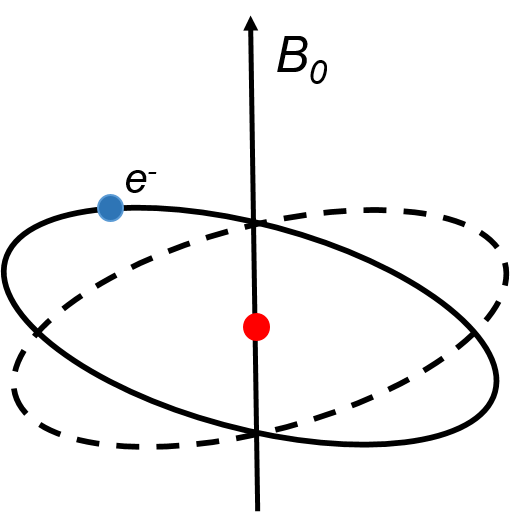
\includegraphics[width = 0.8\textwidth]{diamagnetic_term.png}
				\end{minipage}
			
	\end{itemize}
\end{frame}

	
\begin{frame}{\thesection.\thesubsection. \insertsubsection}
	Let's calculate the effect of ring current in cyclic aromatic molecules. Consider benzene molecule:
	
			\begin{minipage}{0.3\textwidth}
				\begin{figure}
					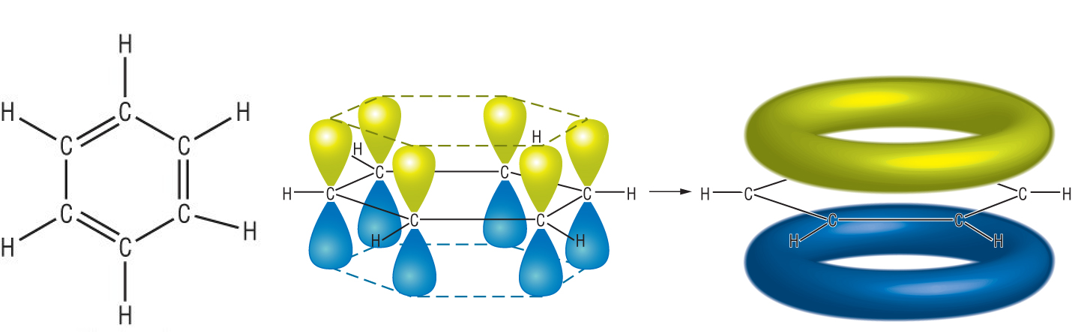
\includegraphics[width=1.0\textwidth]{benzene1.png} \\
					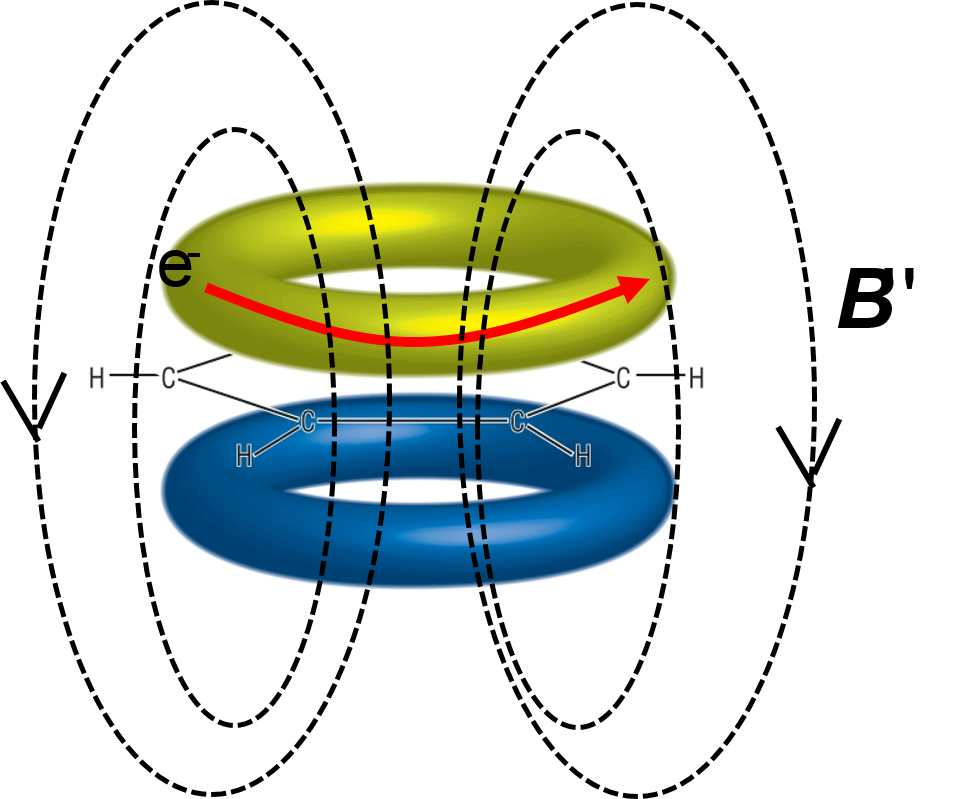
\includegraphics[width=1.0\textwidth]{benzene2.png}
					\caption{(top) Schematic repsresentation of electron orbitals in a benzene molecule, (bottom) local fields in a benzene molecule produced by electron currents induced by a magnetic field.}									
				\end{figure}
				
			\end{minipage}
			\hspace{0.1cm}
			{\tiny
			\begin{minipage}{0.65\textwidth}
				\begin{itemize}[<+>]
					\item
									Larmor precession frequency of electrons $\omega_L = \frac{e B_0}{2 m_e}$. Current can be calculated as charge $6 e$, divided by precession period $\frac{2 \pi}{\omega_L}$:
									\par
									\begin{equation}				    
									i = \dfrac{3e^2 B_0}{2 \pi m_e}
									\end{equation}
					\item 
					Circular conductor creates a magnetic moment $\mu = i \cdot \pi r^2 $, totalling in:				
									\begin{equation}
									\mu = -\dfrac{3 e^2 B_0 r^2}{2 m_e}
									\end{equation}
					\item
									The magnetic field created by a magnetic moment  $\bm{B} = \dfrac{\mu_0}{4 \pi}(\dfrac{\bm{r(mr)}}{r^5} - \dfrac{\bm{m}}{r^3}  )$ reduces to:
									\begin{align}
									B_i = -\dfrac{\mu_0}{4 \pi}\dfrac{m}{r^3} = \dfrac{3 \mu_0 e^2}{8 \pi} \dfrac{r^2}{(r+d)^3} B_0 \\
									\sigma = --\dfrac{\mu_0}{4 \pi m_e}\dfrac{m}{r^3} = \dfrac{3 \mu_0 e^2}{8 \pi} \dfrac{r^2}{(r+d)^3}
									\end{align}
					\item
									Given benzene molecule radius $r=1.4$ \AA, CH-bond length $d = 1.1$ \AA we obtain:
									\begin{equation}
									\sigma \approx -5.3 \cdot 10^{-6}, \sigma_{iso} \approx -1.8 \cdot 10^{-6}
									\end{equation}
					
				\end{itemize}

			\end{minipage}
			
		    }%
			%\caption{(top) Schematic repsresentation of electron orbitals in a benzene molecule, (bottom) local fields in a benzene molecule produced by electron currents induced by a magnetic field.}

		
		
%		\item
%	    In reality there is a diamagnetic and paramagnetic contributions to chemical shift, which can be calculated using quantum mechanics.
%	    
%	    					
%		Diamagnetic shifts arise from $B_0$ induced precession of electron orbitals, which produces a circulating current that slightly reduces the field at the nucleus (shielding).
%		
%		\item	The degree of shielding is proportional to $B_0$ and depends on electron density near nucleusm which is affected by local bonding. It is also affected by bond orientation to the field, but in liquids, the orientation effects are averaged out by molecular motion.
%		
%		\item					
%		Diamagnetic shifts arise from $B_0$ induced precession of electron orbitals, which produces a circulating current that slightly reduces the field at the nucleus (shielding).
%		\item	The degree of shielding is proportional to $B_0$ and depends on electron density near nucleusm which is affected by local bonding. It is also affected by bond orientation to the field, but in liquids, the orientation effects are averaged out by molecular motion.

	
\end{frame}

\begin{frame}{\thesection.\thesubsection. \insertsubsection}
	\begin{itemize}[<+>]
		\item Chemical shifts are usually measured in ppm's and are referenced with respect to the signals of tetramethylsilane (TMS).		
		
		\begin{minipage}[b]{0.15\textwidth}
            \centering
		  	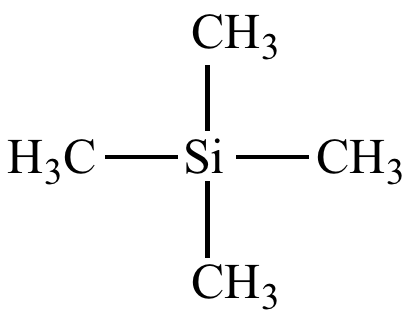
\includegraphics[scale=0.5]{tetramethylsilane.png}	
		\end{minipage}
		\hspace{0.3cm}
		\begin{minipage}[b]{0.7\textwidth}
			{\footnotesize
		 	\begin{align}
		   	\delta = \dfrac{\nu_{sample} - \nu_{TMS}}{\nu_{TMS}}\times 10^{6} \text{ppm} \\
		   	\delta =  (\sigma_{TMS} - \sigma_{sample}) \times 10^{6} \text{ppm}
		   	\end{align}
		   }%	
	    \end{minipage}
			
		
			
		
	
		\item 
		In general the \textsuperscript{1}H chemical shift is greater for nuclei to atoms/bonds that reduce the electron density at the atom. 
		\begin{figure}
		 		\centering
			 	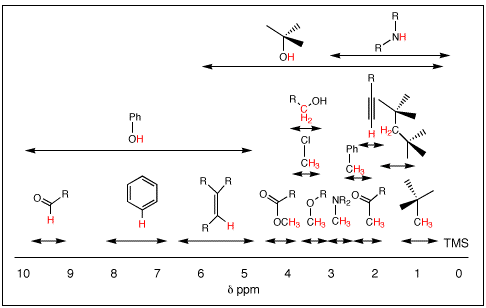
\includegraphics[width=0.50\textwidth]{proton_chemical_shifts.png}
			 	\caption{Chemical shifts in various organic molecules Source: \url{http://orgchem.colorado.edu/Spectroscopy/nmrtheory/protonchemshift.html}}
	 	\end{figure}

	\end{itemize}
	...
\end{frame}


\begin{frame}{\thesection.\thesubsection. \insertsubsection}
	Consider the \textsuperscript{1}H-spectrum of methyl acetate.
	\begin{minipage}{0.4\textwidth}
		\begin{figure}
			\centering
			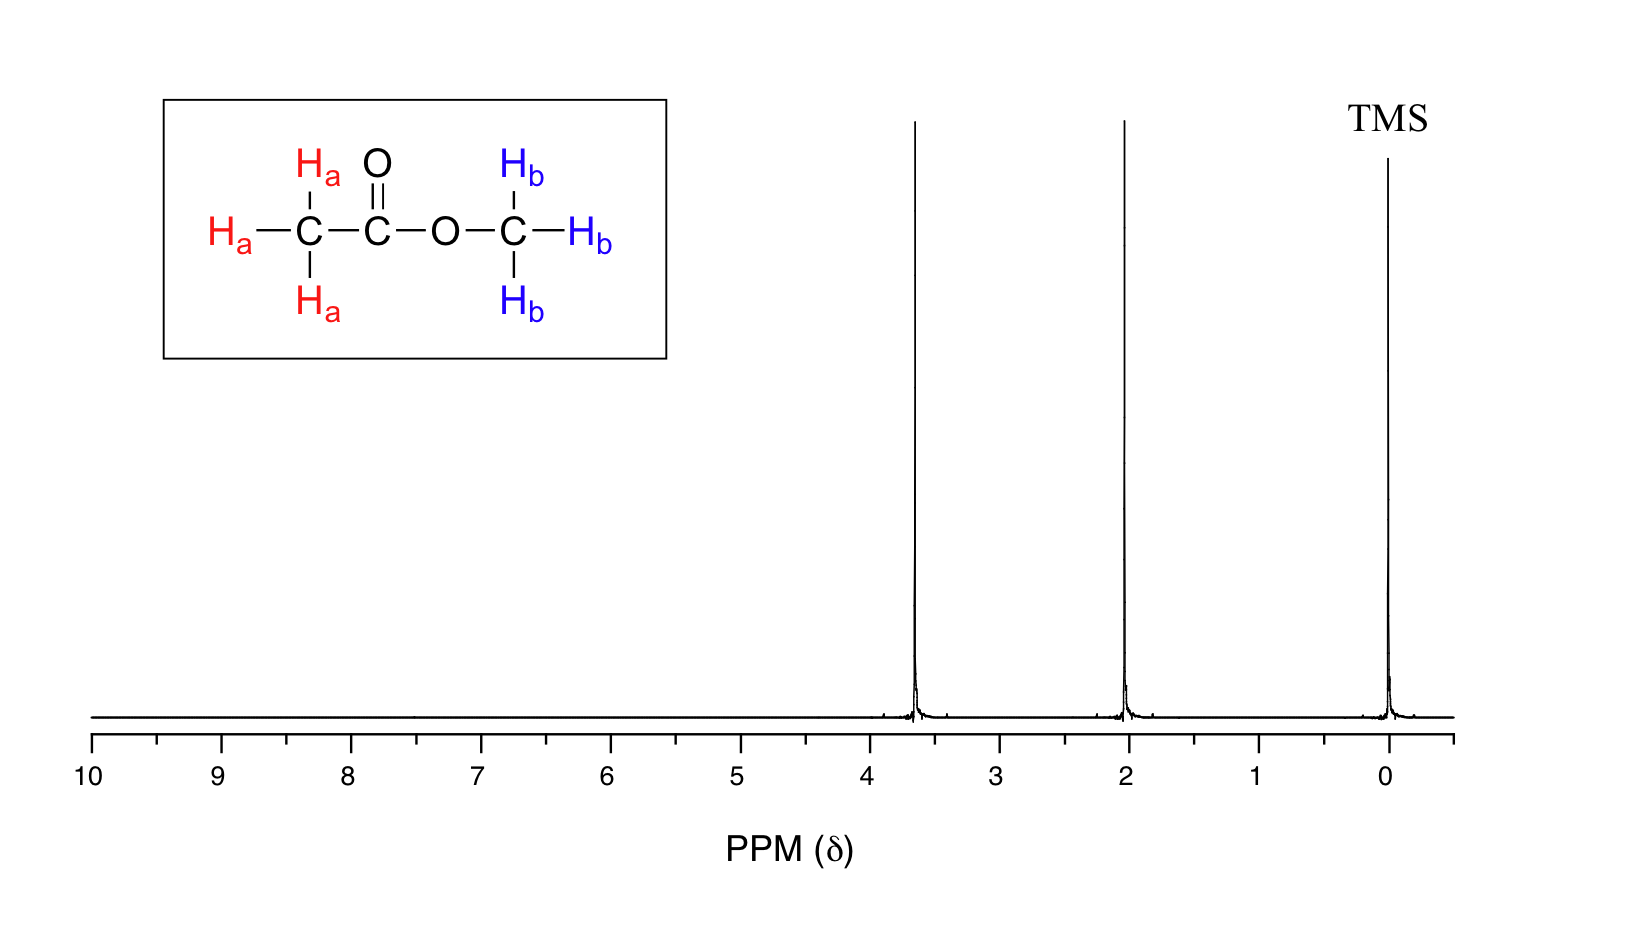
\includegraphics[width=1.0\textwidth]{methyl_acetate.png}
			\caption{\textsuperscript{1}H spectrum of methyl acetate. Source: \url{http://chemwiki.ucdavies.edu/Organic_Chemistry}}
		\end{figure}
    \end{minipage}
    \hspace{0.1cm}
  	\begin{minipage}{0.55\textwidth}
  			\begin{itemize}[<+>]
  				\item the TMS appears at 0 ppm
  				\item chemical shift increases from right to left
  				\item two resonances correpond to protons of the two methyl groups
  				\item the presence of electronegative oxygen atom in methoxy group produces weaker shielding ($\sigma$) thus makes bigger chemical shift $\delta$  
  				\item three nuclei of methyl groups resonate at the same frequency. Peak heights are the same.
  			\end{itemize}  		  		
  		
   	\end{minipage}
   	
\end{frame}
\begin{frame}{\thesection.\thesubsection. \insertsubsection}
	For other nuclei, paramagnetic shifts which arise from mixing of excited state with the ground state dues to the effect of the applicaed field, $B_0$ on the Hamiltonian can be important, and the range of chemical shifts is usully larger than for \textsuperscript{1}H nuclei.
  \begin{figure}
  	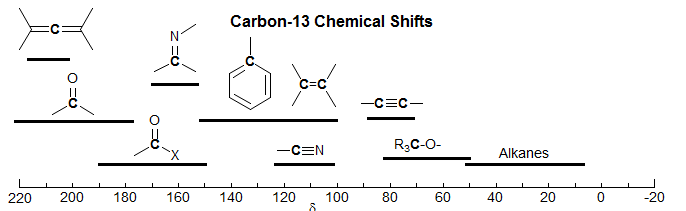
\includegraphics[width=1.0\textwidth]{carbon_chemical_shifts.png}
  	\caption{\textsuperscript{13}C chemical shifts, \url{https://www.chem.wisc.edu/areas/reich/nmr/}}
  \end{figure}	
	
\end{frame}

\subsection{J-couplings.}
\begin{frame}{\thesection.\thesubsection. \insertsubsection}
	Nuclear spins interact with one another. In solution, one prominent spin-spin interaction is called \alert{J-coupling}.
	
	This intra-molecular scalar coupling is caused by the combination of two effects: the Pauli principle means that the electons in the bond have opposite spin-state(spin-up and spin-down), while hyperfine couplings (specifically Fermi contact interaction) meanse that it is energetically favourable for each nuclear spin to be anti-parallel to the electron spin. 
	
  \begin{figure}
  	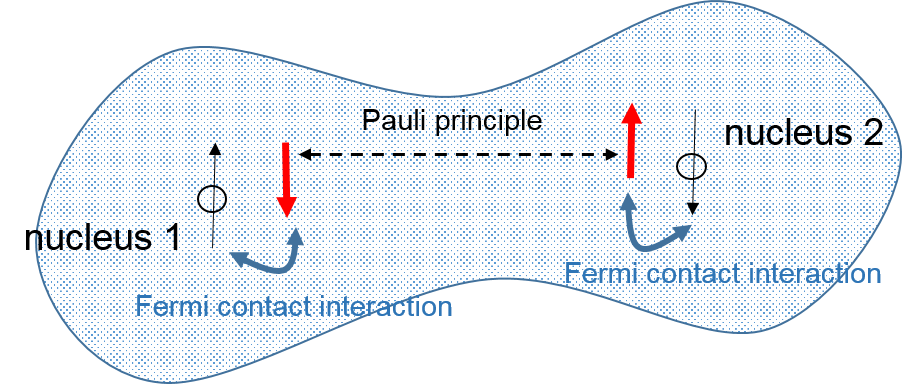
\includegraphics[scale =0.5]{J-coupling.png}
  	\caption{Origin of J-couplings. Low energy configuration in which nuclear spins are antiparallel}
  \end{figure}	

\end{frame}

\begin{frame}{\thesection.\thesubsection. \insertsubsection}
	\begin{itemize}[<+>]
		\item 
			Hamiltonian of J-coupling in solution (all anisotropy is averaged):
			\begin{equation}
			\begin{array}{lcl}
			\hat{H}  &=& J \bm{\hat{I}_{1}} \cdot  \bm{\hat{I}_{2}} = J ( \hat{I}_{1x} \hat{I}_{2x} + \hat{I}_{1y} \hat{I}_{2y} + \hat{I}_{1z} \hat{I}_{2z}   ) =	\\
			&=&  J  \hat{I}_{1z} \hat{I}_{2z} +\dfrac{J}{2} (\hat{I}_{1+} \hat{I}_{2-} + \hat{I}_{1-} \hat{I}_{2+} )  	  
			\end{array}
			\end{equation}
			J is usually measured in units of frequency, i.e. Hz. 
			
		\item
		In frequency units the full spin Hamiltonian for a system of two nuclei A and B of the same kind would be:
		\begin{equation}
		\hat{H} = -\nu_0(1 - \sigma_A) \hat{I}_{Az} - \nu_0(1- \sigma_B) \hat{I}_{Bz} + J  \hat{I}_{Az} \hat{I}_{Bz} +\dfrac{J}{2} (\hat{I}_{A+} \hat{I}_{B-} + \hat{I}_{A-} \hat{I}_{B+} ) 
		\end{equation}
		
	\end{itemize}
		
	
\end{frame}
\begin{frame}{\thesection.\thesubsection. \insertsubsection}
	\begin{itemize}[<+>]
		\item 
		For two coupled spins $\dfrac{1}{2}$ the Hamiltonian matrix in the basis of functions $\vert 1 \rangle =  \vert \alpha_1 \alpha_2 \rangle, \vert 2 \rangle =  \vert \alpha_1 \beta_2 \rangle, \vert 3 \rangle =  \vert \beta_1 \alpha_2 \rangle, \vert 4 \rangle =  \vert \beta_1 \beta_2 \rangle$
		The Hamiltonian matrix of such a system are:
		
		{\tiny
		\begin{equation}
		  H_{ik}= \langle i \vert \hat{H} \vert k \rangle = 
		   \begin{bmatrix}
                 -\dfrac{\nu_A+ \nu_{B}  }{2} + \dfrac{J}{4}   & 0 & 0 & 0 \\
                 0 & -\dfrac{\nu_A-\nu_B}{2} - \dfrac{J}{4}  & \dfrac{J}{2} & 0 \\
                 0 & \dfrac{J}{2} & \dfrac{\nu_A-\nu_B}{2} - \dfrac{J}{4}  & 0 \\
                 0 & 0 & 0 & -\dfrac{\nu_A+\nu_B}{2} + \dfrac{J}{4}                  
		   \end{bmatrix}
		\end{equation}
	    }%
	    when $\mid \nu_A -\nu_B \mid \gg J $ the off-diagonal terms due to $\hat{I}_{A\pm} \hat{I}_{B\mp}$ can be neglected. That is a called \alert{AX system}. When off-diagonal terms cannot be neglected, we deal with a so called \alert{AB system}.
	
		\item 
		
		Let's consider nuclei of the same type (i.e. both \textsuperscript{1}H or both \textsuperscript{13}C ). When $\gamma_N \hbar \mid \omega_1 -\omega_2 \mid \ll J $,
		
	\end{itemize}
	
	
\end{frame}

\subsection{J-couplings in AX system.} \label{sec: J-couplings in AX system}
\begin{frame}{\thesection.\thesubsection. \insertsubsection}
      Eq.\ref{eq:probability} is non-zero when corresponding matrix element is not zero. The selection rules for two nuclei then  : $\langle i \vert \hat{I}_{1x} + \hat{I}_{2x} \vert k \rangle \neq 0 $. 
		
		\begin{figure}[ht]
				\centering
				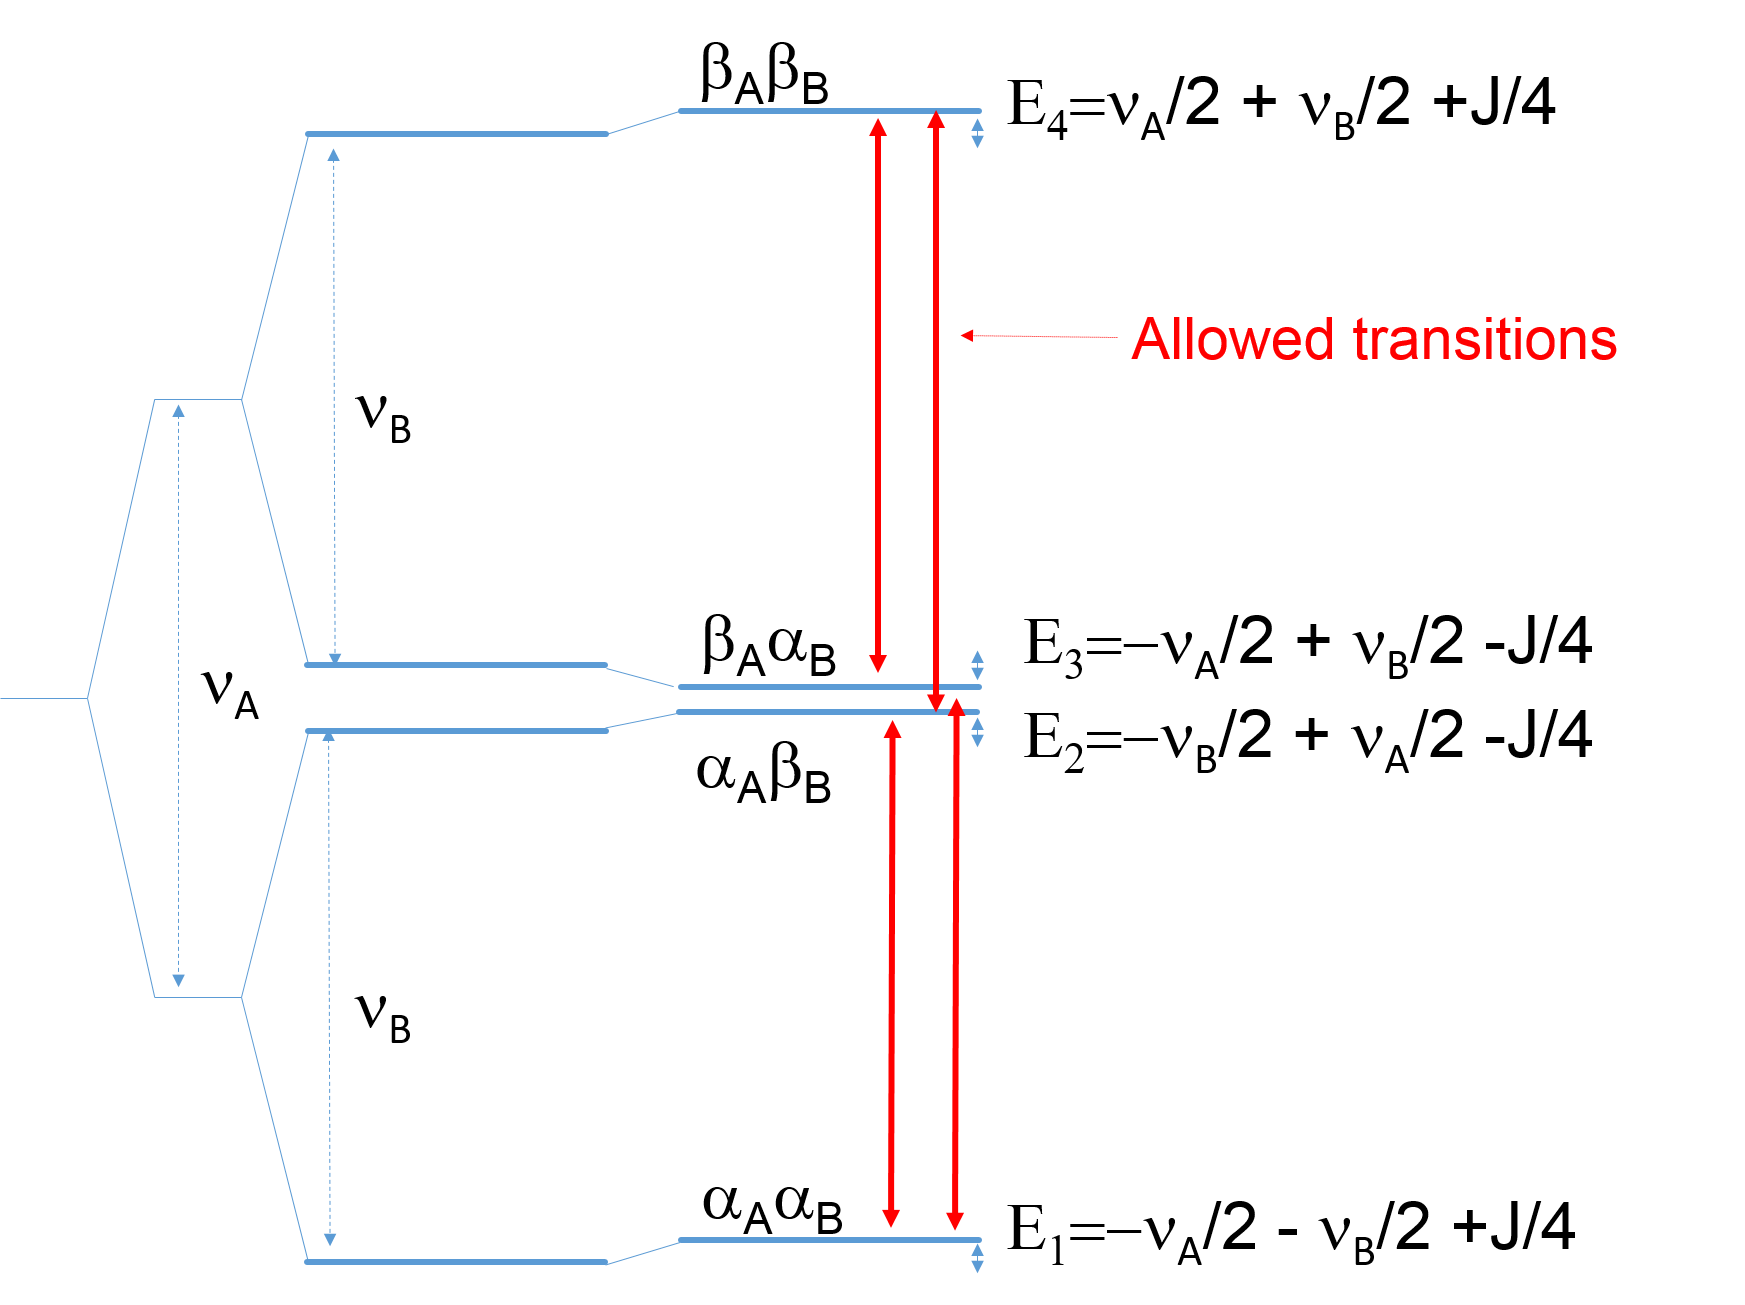
\includegraphics[width=0.8\textwidth]{AXsystem.png}
				\caption{Level diagram for two J-coupled spins in AX system}
				\label{fig1}

		\end{figure}
	
	
	...
\end{frame}

\begin{frame}{\thesection.\thesubsection. \insertsubsection}
  In a more general case, when $I_A, I_B \neq \dfrac{1}{2}$, the energy levels follow the following equation:
  	\begin{equation}
  	E =  -\nu_A m_1 - \nu_0(1- \sigma_B) m_2 + J  m_1 m_2 
  	\end{equation}
  	The allowed transitions for spin $A$ have the following frequencies:
  	\begin{equation}
  	   \nu = \nu_A + m_B J,
   	\end{equation}
   	where $m_B = -I_B, -(I_B-1) ... (I_B-1), I_B $ is the projection of nuclear spin $B$. The resonance line is therefore being split into several components. 
   	Similarly, for spin $B$:
   	\begin{equation}
  	   \nu = \nu_B + m_A J,
   	\end{equation}
  
\end{frame}

\subsection{Interpreting simple NMR spectra}
\begin{frame}{\thesection.\thesubsection. \insertsubsection}
For one coupled nucleus:
\begin{equation}
\nu = \nu_A + m_B J,
\end{equation}
For two coupled nuclei:
\begin{equation}
\nu = \nu_A + m_B J + m_C J  ,
\end{equation}
For three:
\begin{equation}
\nu = \nu_A + m_B J + m_C J + m_D J  ,
\end{equation}


\begin{figure}
		\centering
		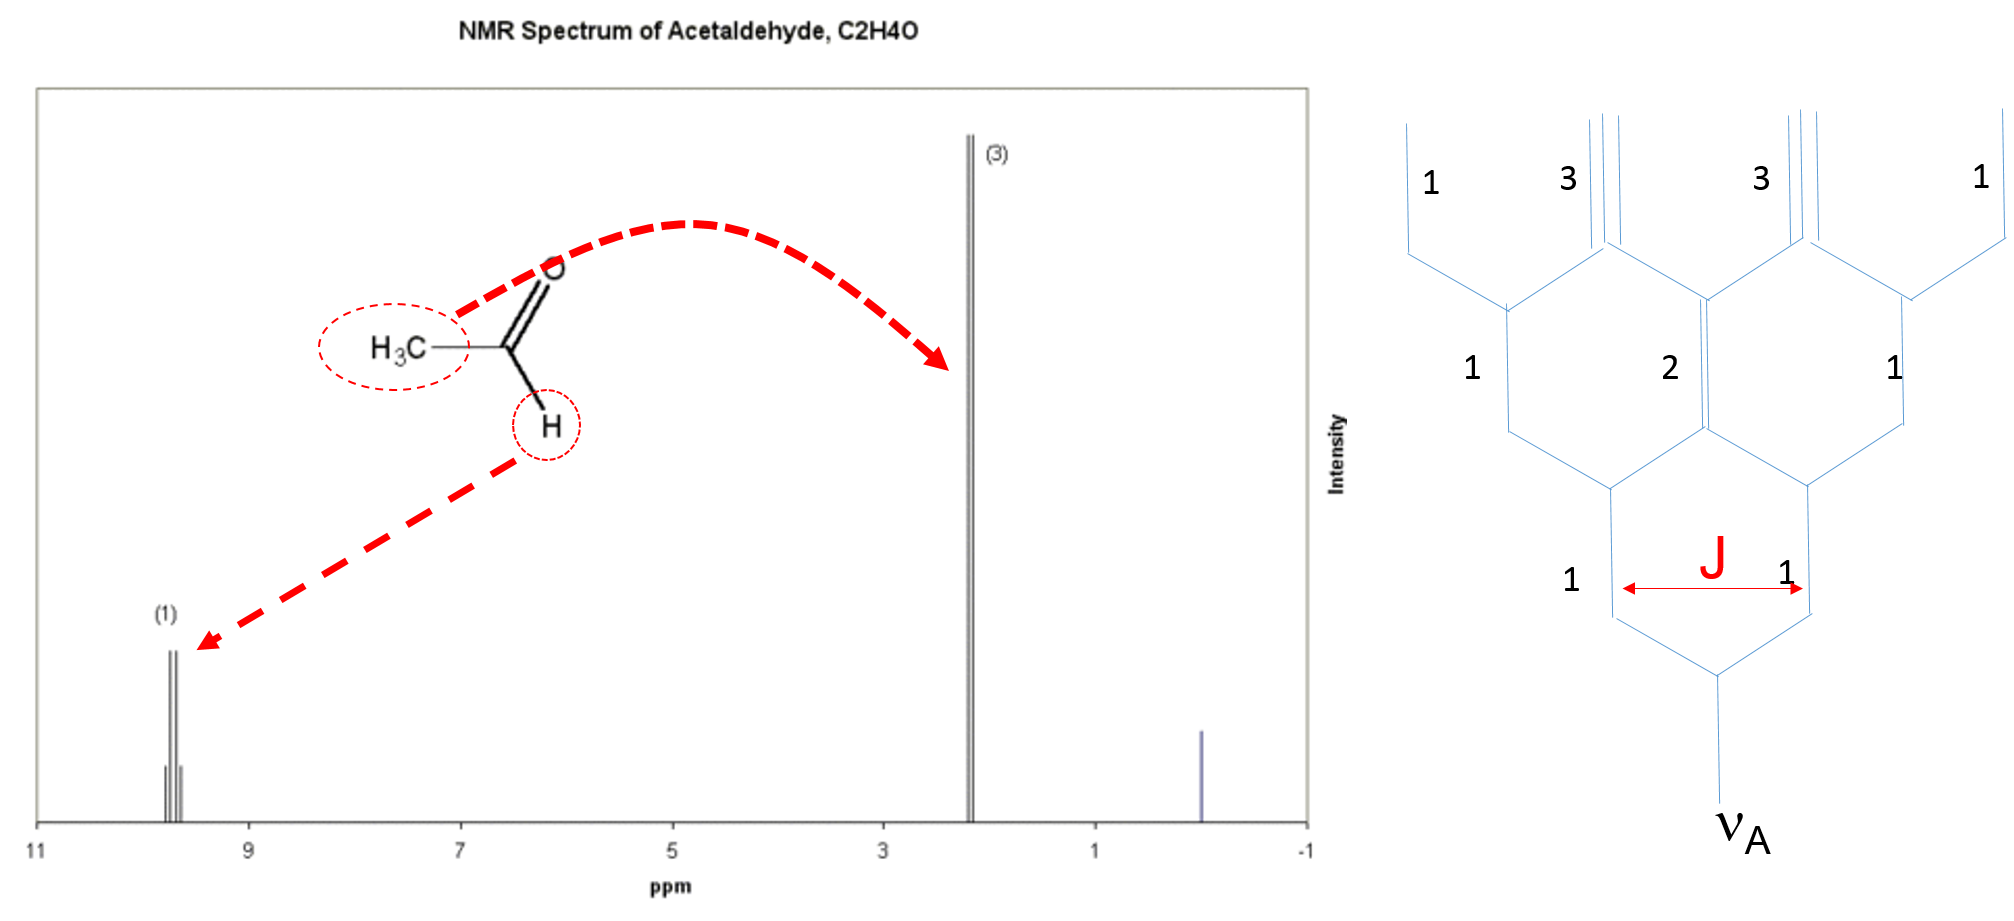
\includegraphics[scale = 0.2]{nmracetaldehyde.png}
		\caption{Spectrum of acetaldehyde. Source: \url{https://chem242.wikispaces.com}}
		\label{fig1}
\end{figure}	
	
	
\end{frame} 	
  
\begin{frame}{\thesection.\thesubsection. \insertsubsection}
	\begin{block}{Problem}
	  Draw schematically  \textsuperscript{1}H spectrum of ethyl alcohol?  Proton Larmor frequency is 90 MHz (i.e. treat as AX system).

	\end{block}
	\begin{itemize}[<+>]
		\item[] 
		    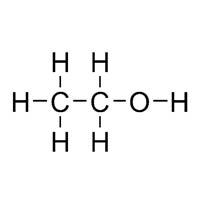
\includegraphics[scale=0.2]{ethyl_alcohol.jpg} \\
		    $\delta_{CH3}=1.22$ ppm, $\delta_{CH2}=3.68$ ppm, $\delta_{OH}=2.61$ ppm, consider only $J_{CH2-CH3}=7.29$ Hz.
		 \item[] 
		 \begin{figure}
		     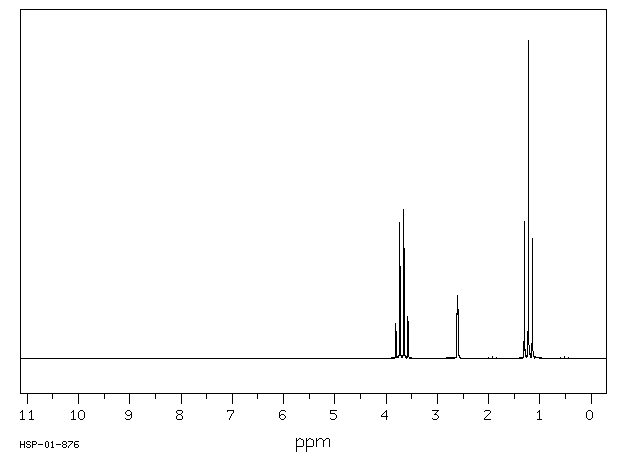
\includegraphics[scale=0.2]{ethyl_alcohol_nmr.png}  
		     \caption{Ethanol spectrum at 90 MHz in CDCl \textsubscript{3}}
		 \end{figure}
	\end{itemize}
\end{frame}

\subsection{Range of J-couplings. Are they useful for structure determination?}

\begin{frame}{\thesection.\thesubsection. \insertsubsection}
	\begin{figure}
		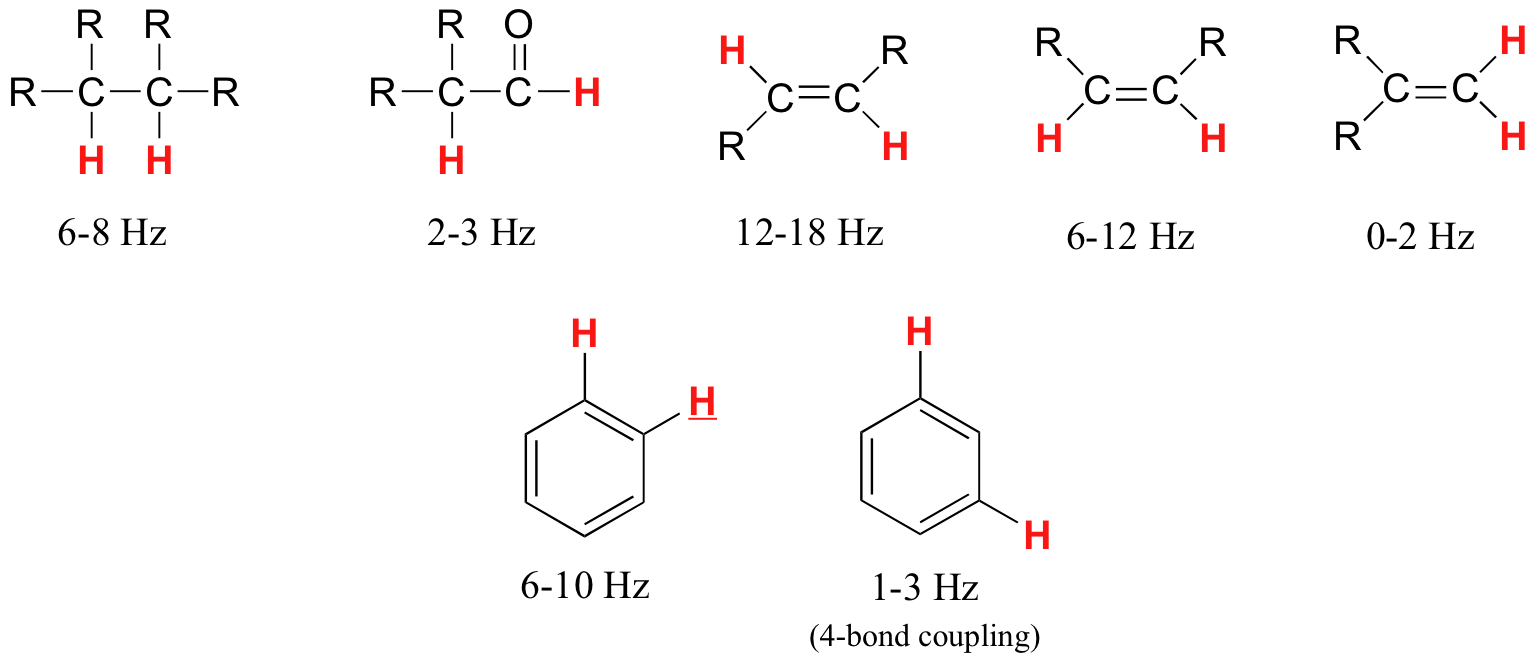
\includegraphics[scale=0.4]{j-couplings.png}
		\caption{Typical J-couplings \url{	https://chem.libretexts.org/Textbook_Maps/Organic_Chemistry_Textbook_Maps/}}
	\end{figure}
   {\small
   Is there any simple meaning to J-couplings? \alert{Karplus equation} is an empiric formula for $J$ coupling as a function of a dihedral angle $\phi$. 
   }%
	
   \begin{minipage}[t]{0.4\textwidth}
   	   \begin{equation}
   	   J = A \cos \phi + B \cos 2\phi + C
   	   \end{equation}   	      	
   \end{minipage}
   \hspace{0.1cm}
   \begin{minipage}[t]{0.5\textwidth}
   	\begin{figure}
   		\centering
   		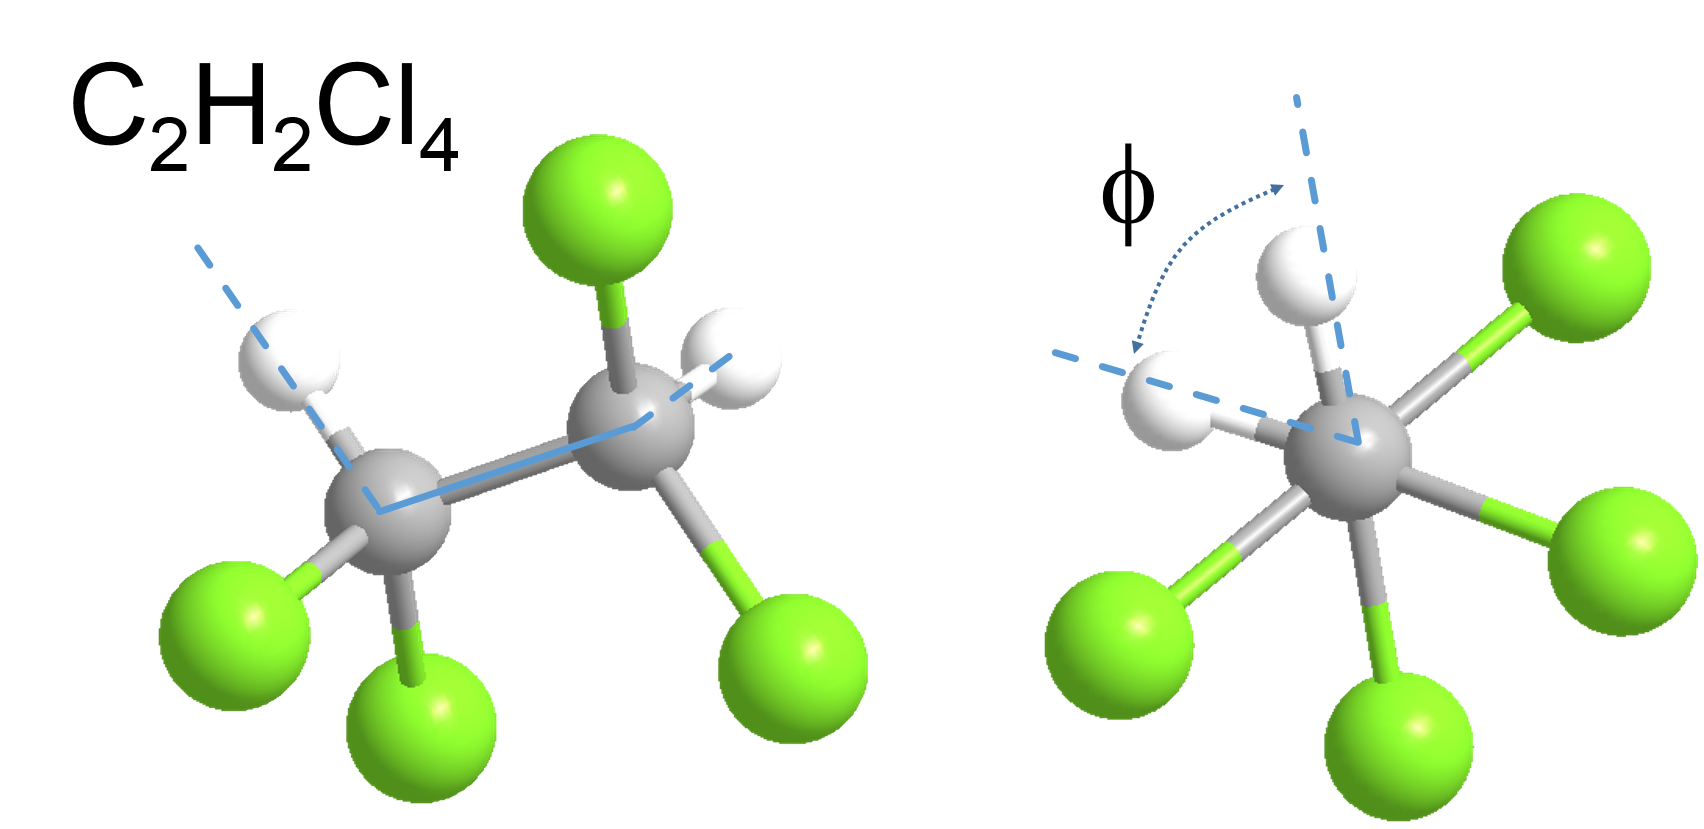
\includegraphics[scale = 0.12]{C2H2Cl4.png}
   		\caption{Dihedral angle in 1,1,2,2-tetrachlorethane}
   		\label{fig1}
   	\end{figure}   	
   \end{minipage}
      


   

\end{frame}

\subsection{Heteronuclear J-couplings.}

\begin{frame}{\thesection.\thesubsection. \insertsubsection}
  Heteronuclear systems are automatically AX systems, i.e. $\mid \nu_A - \nu_B \mid \gg J$. \\
  Example: trifluromethane (fluoroform) \\
  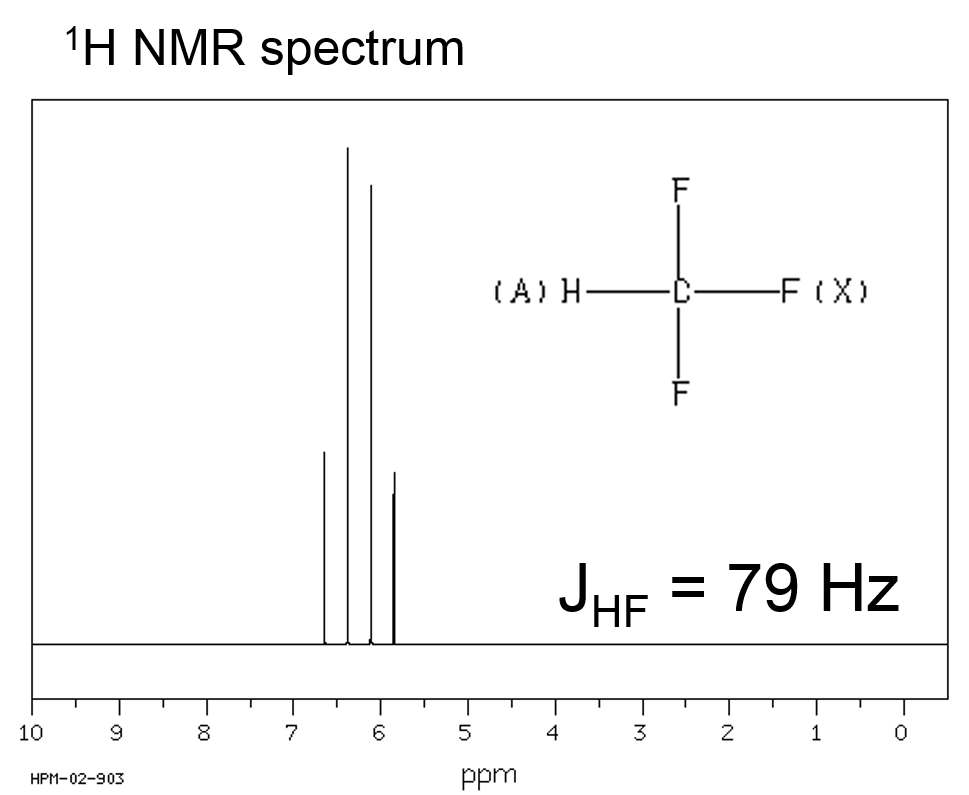
\includegraphics[scale = 0.5]{CF3H.png}
  
\end{frame}

\begin{frame}{Summary of lecture 3.}
	\begin{itemize}
		\item J-couplings and chemical shift to an extent are unique in different molecules, and NMR spectra help in identifying chemical compounds by their spectra.
		\item Chemical shifts originate from magnetic field shielding by electrons.
		\item CS report on the chemical environment of a nucleus
		\item J-couplings cause spectral splittings. \\
		\textbf{Suggested reading: } Harris 1.8, 1.9, 1.11, 1.12, 1.13, 8.2, 8.9., 8.23 \\
		For more detailed quantum mechanical theory of chemical shifts: Slichter 4.1-4.5, for detailed theory of J-couplings: Slichter 4.9 
	\end{itemize}
\end{frame}

\subsection{J-coupling in equivalent system.}
\begin{frame}{\thesection.\thesubsection. \insertsubsection}

Are protons in CH3 or CH2 groups coupled to one another? \\
\textbf{Yes.} But they are equivalent and therefore not observed.

\begin{itemize}[<+>]
	\item 
	
	\begin{equation}
	\hat{H} = - \nu_0 (\hat{I}_{1z} + \hat{I}_{2z}+ \hat{I}_{3z}) + J (\bm{I}_1 \bm{I}_2 + \bm{I}_2 \bm{I}_3  + \bm{I}_1 \bm{I}_3 )
	\end{equation}
	
	\item
	Let's rewrite the last term as:
	\begin{equation}
	\bm{I}_1 \bm{I}_2 + \bm{I}_2 \bm{I}_3  + \bm{I}_1 \bm{I}_3 = \dfrac{1}{2} (\bm{I}_1 + \bm{I}_2 + \bm{I}_3 )^2 - \dfrac{1}{2} ( \bm{I}_1^2 + \bm{I}_2^2 + \bm{I}_3^2)
	\end{equation}
	
	\item	
	We can introduce new operator: $\bm{F} =\bm{I}_1 + \bm{I}_2 + \bm{I}_3$. Given that $I_1=I_2=I_3=\dfrac{1}{2}$ the Hamiltonian can be rewritten using this new operator:
	\begin{equation}
	\hat{H} = - \nu_0 \hat{F}_{z} + J (\bm{F}^2 - \dfrac{9}{4} )    
	\end{equation}
	
	\item	
	Eigenfunctions of this Hamiltonian are functions $\vert F M_F \rangle$, where $F=\dfrac{1}{2}$ or $\dfrac{3}{2}$.
\end{itemize}

\end{frame}
\begin{frame}{\thesection.\thesubsection. \insertsubsection}

\begin{itemize}[<+>]
	\item
	
	\begin{equation}\label{eq:equivalennce}
	\hat{H} = - \nu_0 \hat{F}_{z} + J (\bm{F}^2 - \dfrac{9}{4} )    
	\end{equation}
	
	Selection rules for transitions: $\langle i \vert  \hat{F}_x \vert k \rangle \neq 0$, since $\hat{F}_x = \dfrac{\hat{F}_{+} + \hat{F}_{-}}{2}$, the selection rules then are: $\langle i \vert  \hat{F}_{\pm} \vert k \rangle \neq 0$
	Since $\hat{F}_{\pm} = const \vert F M_F\pm1 \rangle$, the allowed transition does not change the second term in Eq.\ref{eq:equivalennce}.
	
	\item
	Strictly speaking if a molecule contains only nuclei of one type, and no other $J$-splitting will not be observed. Examples: tetramethylsilane (TMS), benzene
    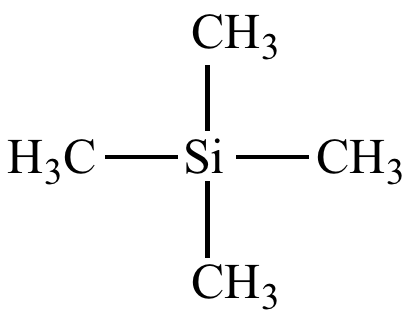
\includegraphics[scale = 0.5]{tetramethylsilane.png}
    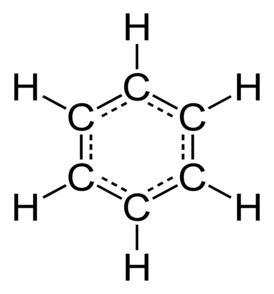
\includegraphics[scale = 0.15]{Benzene-2D-flat.png}
\end{itemize}
\end{frame}

\begin{frame}{\thesection.\thesubsection. \insertsubsection}
	\begin{block}{Problem}
		Sketch the \textsuperscript{1}H NMR spectra of 2,3-dibromothiophene and 2,5-dibromothiophene?  \textsuperscript{79}Br and \textsuperscript{81}Br are quadrupolar nuclei, and their J-couplings can be ignored.\\
		\centering
		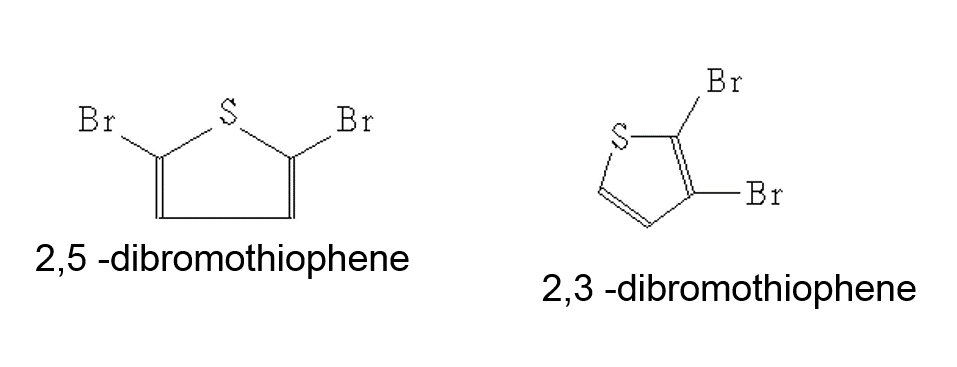
\includegraphics[scale=0.3]{DBTproblem1.png}
	\end{block}
\end{frame}

\begin{frame}{\thesection.\thesubsection. \insertsubsection}
	\centering
	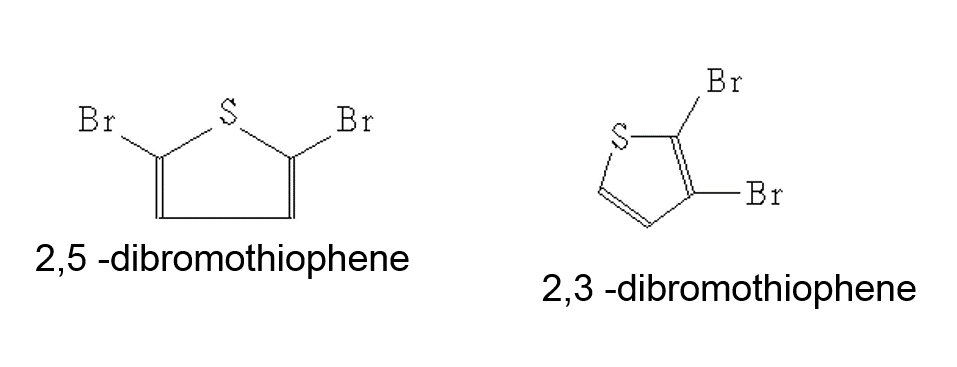
\includegraphics[scale=0.4]{DBTproblem1.png}\\
	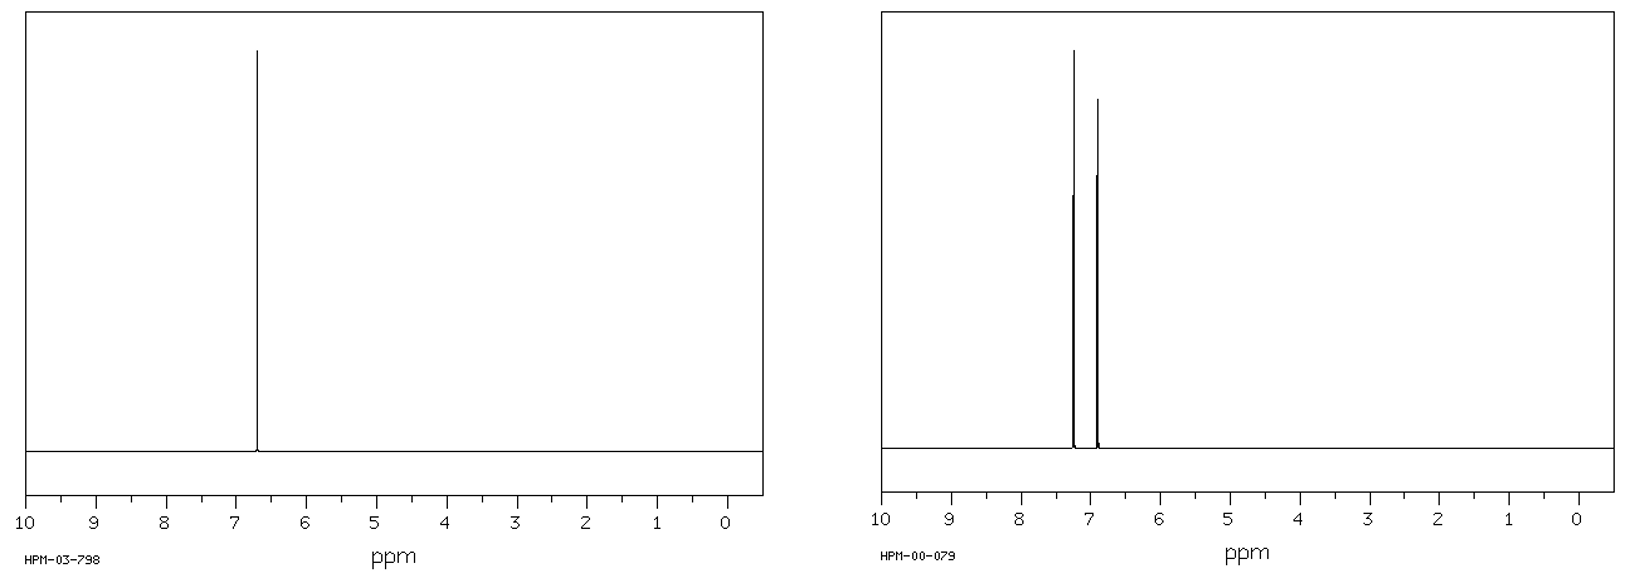
\includegraphics[scale=0.4]{DBTproblem2.png}
	
\end{frame}


\subsection{J-coupling in AB system.}
\begin{frame}{\thesection.\thesubsection. \insertsubsection}
	What happens if $\nu_A - \nu_B \gg J$ is no longer true?
	
	\begin{itemize}[<+>]
		\item 
		The matrix of spin Hamiltonian is:
		
			
			{\tiny
				\begin{equation}				
				\begin{bmatrix}
				-\dfrac{\nu_A+ \nu_{B}  }{2} + \dfrac{J}{4}   & 0 & 0 & 0 \\
				0 & -\dfrac{\nu_A-\nu_B}{2} - \dfrac{J}{4}  & \dfrac{J}{2} & 0 \\
				0 & \dfrac{J}{2} & \dfrac{\nu_A-\nu_B}{2} - \dfrac{J}{4}  & 0 \\
				0 & 0 & 0 & -\dfrac{\nu_A+\nu_B}{2} + \dfrac{J}{4}                  
				\end{bmatrix}
				\end{equation}
			}%
		\item The general way of solving is finding the eigenvalues and eigenvalues and eigenfunctions of this Hamiltonian.
		\item
		the solution can be represented by following replacements:
		\begin{equation}
		\begin{array}{l}
		\dfrac{\nu_A - \nu_B}{2} = \dfrac{\delta}{2} = C \cos 2\theta \\
		\dfrac{J}{2} = C \sin 2\theta \\
		C = \dfrac{1}{2}\sqrt{\delta^2 + J^2}, \tan 2\theta = \dfrac{J}{\delta}, \bar{\nu} = \dfrac{\nu_A + \nu_B}{2}
		\end{array}
		\end{equation}
	\end{itemize}
\end{frame}

\begin{frame}{\thesection.\thesubsection. \insertsubsection}
	  In this notation the eigenvalues and eigenfunctions are:
	  {\small
	  	\begin{equation}
	  	\begin{array}{ll}
	  	E_1 = -\bar{\nu}+\dfrac{J}{4} & \phi_1 = \vert \alpha_A \alpha_B \rangle \\
	  	E_2 = -\dfrac{J}{4} - C & \phi_2 =  \sin \theta \vert \alpha_A \beta_B \rangle - \cos \theta \vert \beta_1 \alpha_2 \rangle \\
	  	E_3 = -\dfrac{J}{4} + C & \phi_2 =  \cos \theta \vert \alpha_A \beta_B \rangle + \sin \theta \vert \beta_1 \alpha_2 \rangle \\
	  	E_4 = \bar{\nu} + \dfrac{J}{4}& \phi_4 = \vert \beta_A \beta_B \rangle 
	  	\end{array}
	  	\end{equation}
	  }%
	    \begin{minipage}[t]{0.65\textwidth}
	    	\begin{figure}
	    		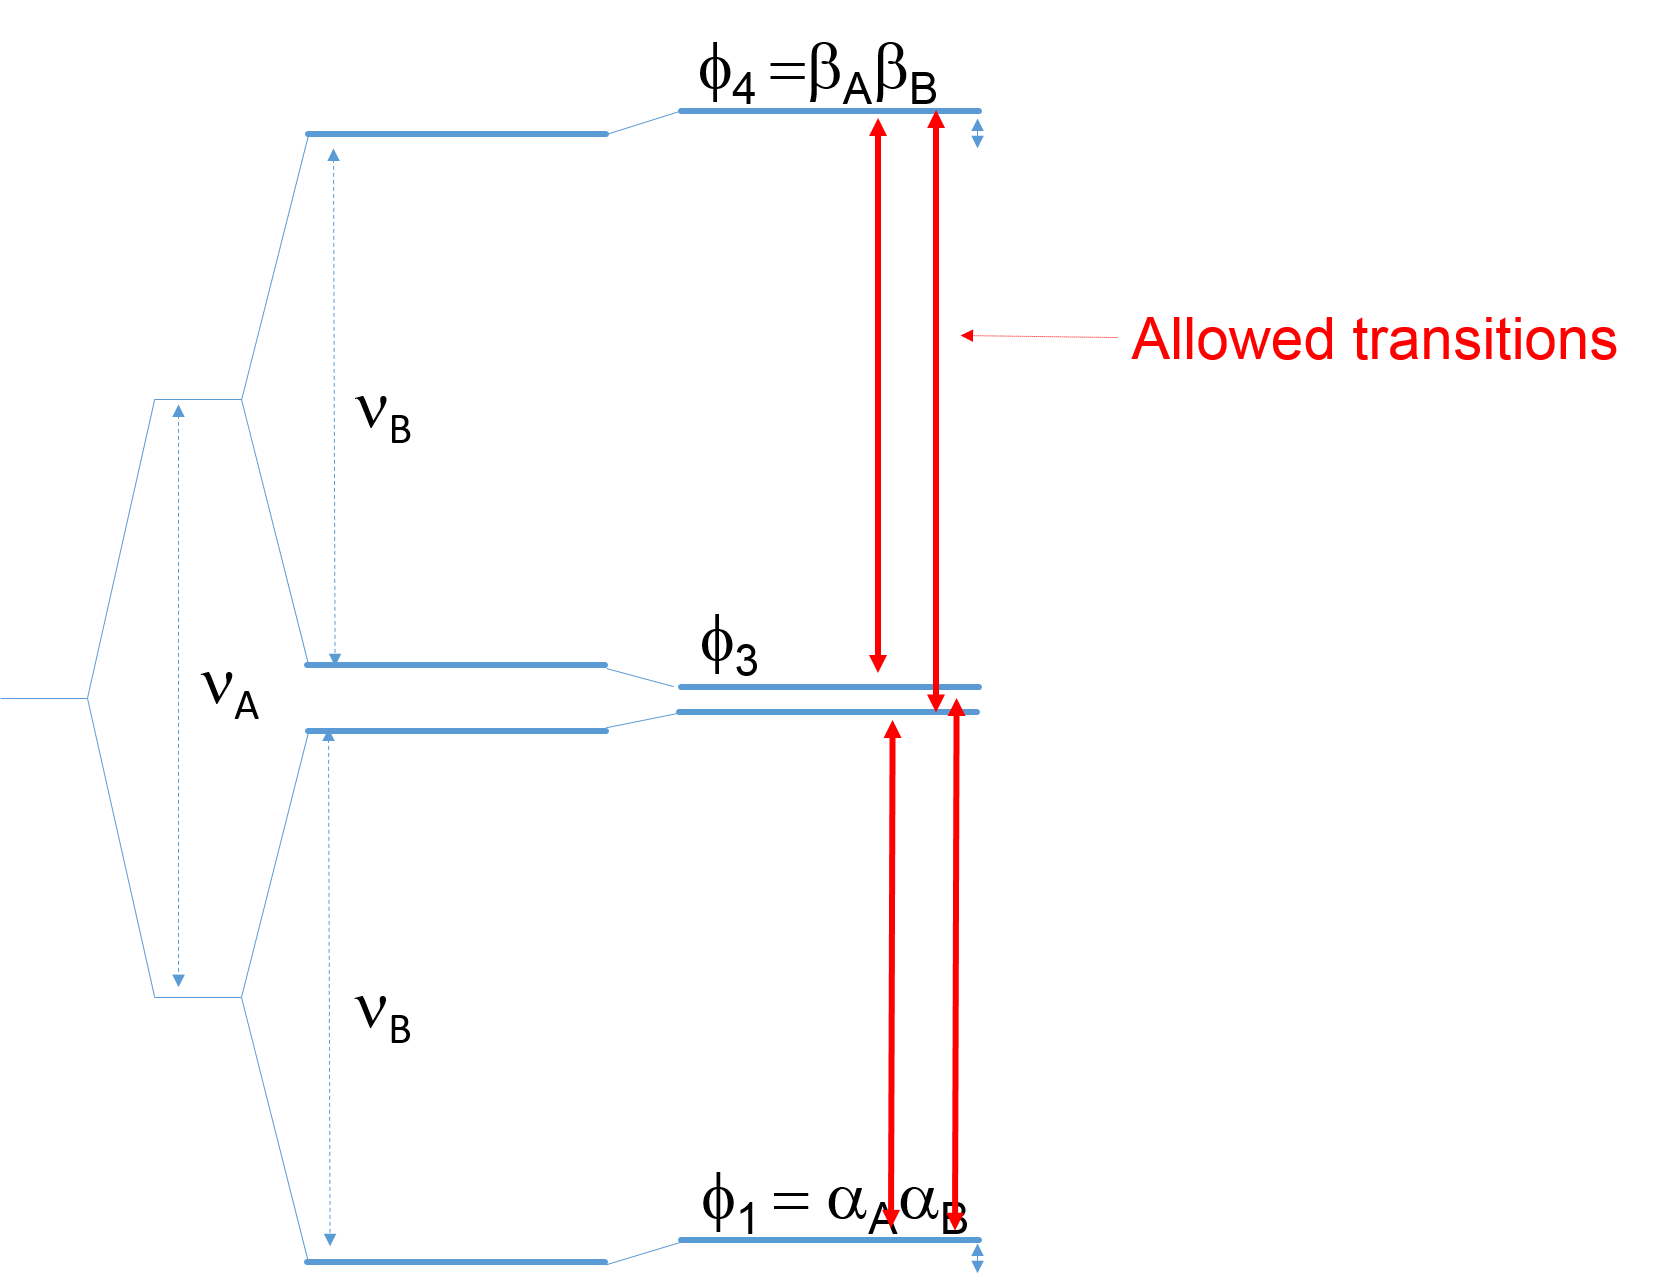
\includegraphics[scale=0.2]{ABsystem.png}
	    		\caption{Level diagram for AB system of J-coupled nuclei.}
	    	\end{figure}
	    \end{minipage}
	    \hspace{0.1cm}
	    \begin{minipage}[t]{0.3\textwidth}
	    	\begin{block}{Problem}
               Calculate the transition probability between levels 1 and 2?(Hint: use Eq.\ref{eq:probability} )
	    	\end{block}	    	
	    \end{minipage}	   	  

\end{frame}
\begin{frame}{\thesection.\thesubsection. \insertsubsection}
  \begin{block}{Problem}
     Calculate the transition probability between levels 1 and 2?(Hint: use Eq.\ref{eq:probability} )
  \end{block}	    	
  For transition $1 \leftrightarrow 2$ we have:
  \begin{equation}
  \begin{split}
      I_{1 \leftrightarrow 2} &\sim \mid \langle 1 \vert \hat{I}_{Ax} + \hat{I}_{Bx} \vert 2 \rangle  \mid^2 = \\
      &= \langle 1 \vert \dfrac{\hat{I}_{A+} + \hat{I}_{A-}}{2}  + \dfrac{\hat{I}_{B+} + \hat{I}_{B-}}{2}   \vert 2 \rangle ^2 =\\
      &= \Big( \langle \alpha_A  \alpha_B  \vert \dfrac{\hat{I}_{A+} + \hat{I}_{A-}}{2}  + \dfrac{\hat{I}_{B+} + \hat{I}_{B-}}{2}   \vert  \sin \theta \vert \alpha_A \beta_B  \rangle + \cos \theta \vert  \beta_A \alpha_B  \rangle  \Big) ^2 =\\
      &= \Big( \dfrac{\cos \theta + \sin \theta}{2}    \Big)^2 = \dfrac{1 + \sin 2\theta}{4}
  \end{split}
  \end{equation}
\end{frame}


\begin{frame}{\thesection.\thesubsection. \insertsubsection}
For all the transitions we obtain:
{\tiny
	\begin{center}
		\begin{tabular}{ccc}
			Transition & Frequency & Intensity: \\ \hline
			$4 \leftrightarrow 2$  & $\bar{\nu}+C+\dfrac{J}{2} $ & $ \dfrac{1-\sin 2 \theta}{4}$ \\
			$3 \leftrightarrow 1$  & $\bar{\nu}+C-\dfrac{J}{2} $ & $ \dfrac{1+\sin 2 \theta}{4}$ \\
			$4 \leftrightarrow 3$  & $\bar{\nu}-C+\dfrac{J}{2} $ & $ \dfrac{1+\sin 2 \theta}{4}$ \\
			$2 \leftrightarrow 1$  & $\bar{\nu}-C-\dfrac{J}{2} $ & $ \dfrac{1-\sin 2 \theta}{4}$ \\			         
		\end{tabular}
	\end{center}
}%

\begin{figure}\label{fig:dibromethiophene}
	\centering
	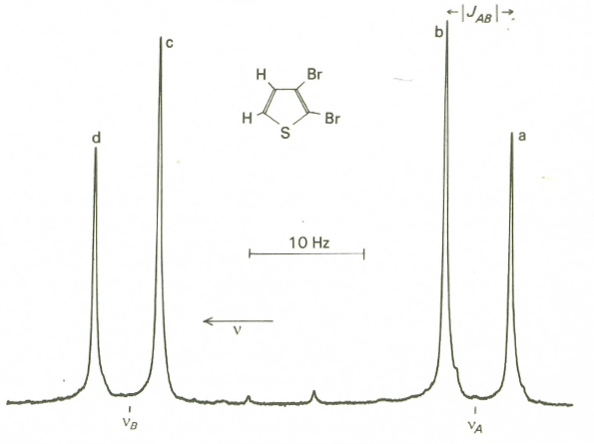
\includegraphics[scale=0.25]{bromothiophene.png}
	\caption{100 MHz \textsuperscript{1}H NMR spectrum of 2,3-dibromothiophene, $\mid \nu_A-\nu_B  \mid = 30.5$ Hz, $J= 5.7$ Hz}
\end{figure}

\end{frame}




\begin{frame}{\thesection.\thesubsection. \insertsubsection}
	For all the transitions we obtain:
	{\tiny
	\begin{center}
		\begin{tabular}{ccc}
           Transition & Frequency & Intensity: \\ \hline
           $4 \leftrightarrow 2$  & $\bar{\nu}+C+\dfrac{J}{2} $ & $ \dfrac{1-\sin 2 \theta}{4}$ \\
           $3 \leftrightarrow 1$  & $\bar{\nu}+C-\dfrac{J}{2} $ & $ \dfrac{1+\sin 2 \theta}{4}$ \\
           $4 \leftrightarrow 3$  & $\bar{\nu}-C+\dfrac{J}{2} $ & $ \dfrac{1+\sin 2 \theta}{4}$ \\
           $2 \leftrightarrow 1$  & $\bar{\nu}-C-\dfrac{J}{2} $ & $ \dfrac{1-\sin 2 \theta}{4}$ \\			         
		\end{tabular}
	\end{center}
    }%
    {\tiny
    Consider following scenarios:\\
    1.  $J \ll \delta$ means that $\sin 2\theta \ll 1$ and $C \approx \dfrac{\delta}{2}$. The leads to AX system shown Fig.\ref{fig:AXABcouplings}B  \\
    2. $\delta \ll J$ means that $\sin 2\theta \approx 1$. A strong double and two weak sattelite lines in Fig.\ref{fig:AXABcouplings}C. 
    }%
	\begin{figure}\label{fig:AXABcouplings}
		\centering
		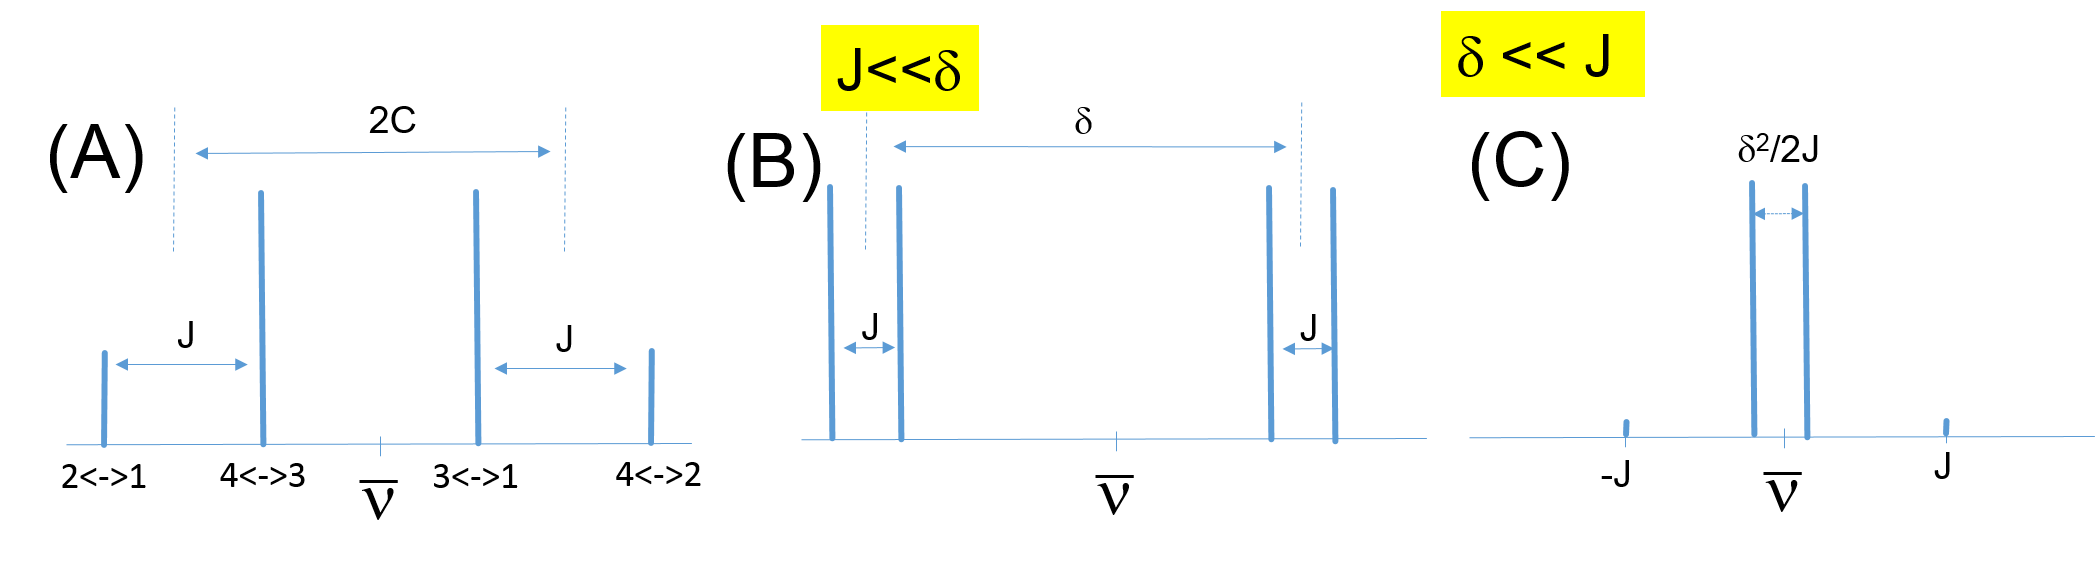
\includegraphics[scale=0.25]{ABspectra.png}
		\caption{Schematic spectra in  several cases (A) $\mid \nu_A - \nu_B \mid \sim J$ ,(B) weakly coupled nuclei $\mid \nu_A - \nu_B \mid \gg J$ , (C) very weak J-coupling $\mid \nu_A - \nu_B \mid \ll J$ }
	\end{figure}
	
	
\end{frame}

\begin{frame}{\thesection.\thesubsection. \insertsubsection}
	\begin{figure}
		\centering
		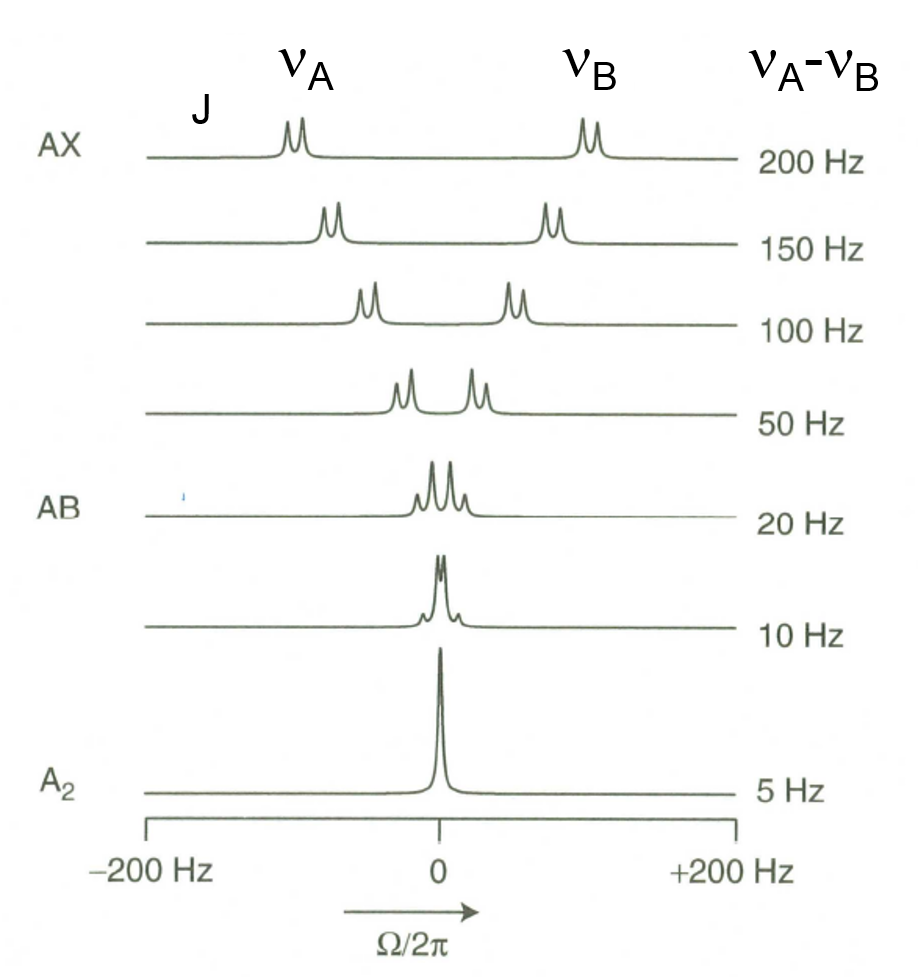
\includegraphics[scale=0.4]{ABspectra2.png}
		\caption{Spectra of spin $\dfrac{1}{2}$ pairs for $J = 10$ Hz as a function of Larmor frequency difference.}
	\end{figure}	
\end{frame}

\begin{frame}{Summary of Lecture 4.}
	\begin{itemize}
		\item Splittings in equivalent systems are not observed.
		\item The case of strong J-couplings can be treated exactly.\\
	\end{itemize}
    \textbf{Suggested reading: } Harris 1.14, 2.17, 2.10 \\
\end{frame}

\section{NMR spectra of solids.}
\subsection{Dipolar coupling.}


\begin{frame}{\thesection.\thesubsection. \insertsubsection}
	\begin{itemize}[<+>]
		\item Nuclear magnetic moments of nuclei interact via dipolar interaction. (It is averaged to zero in liquids). Classical expression for such interaction is:
		
		\begin{minipage}[t]{0.45\textwidth}
			\begin{align*}
			&E  = -(\bm{m_1} \bm{B_{dip}})=  \\
			 &=\dfrac{\mu_0}{4 \pi} \Big(  \dfrac{ 3 (\bm{m_1}  \bm{r})  (\bm{m_2} \bm{r}) }{r^5} - \dfrac{  \bm{m_1} \bm{m_2}}{r^3}  \Big),
			\end{align*}
			
		\end{minipage}
		\hspace{0.1cm}
		\begin{minipage}[t]{0.40\textwidth}
			\begin{figure}
				\centering
				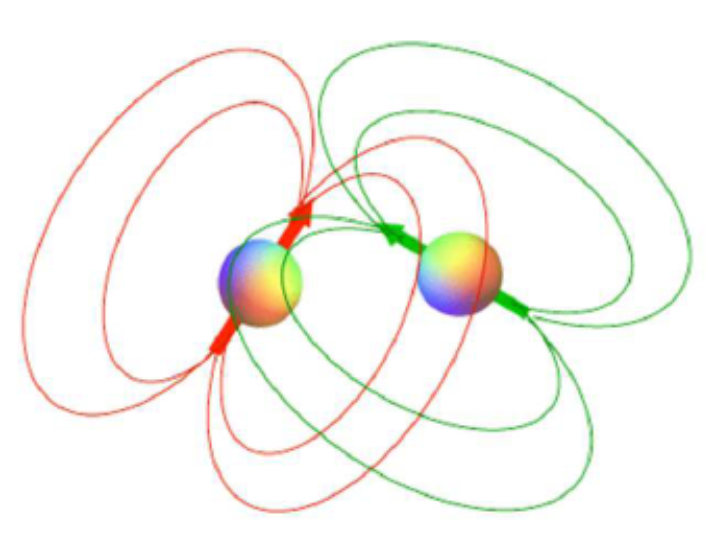
\includegraphics[scale=0.1]{dipolar_fields.png}
			\end{figure}
    	\end{minipage}
		
		\item The field induced by another one proton at the location of other proton spaced apart by 1.6 \AA  is $B_{dip} \sim \dfrac{m}{r^3} \approx 0.7$mT or $\dfrac{g_N \beta_N B_{dip}}{2 \pi \hbar} \approx 30$ kHz.
				
		
		\item In quantum mechanics the magnetic moments $\bm{m_1}$,$\bm{m_2}$ are replaced with operators  $g_{1,2} \beta_{1,2} \hat{I}_{1,2} = \gamma_{1,2} \hbar \hat{I}_{1,2}$, giving rise to a spin Hamiltonian of dipolar interaction:
		\begin{equation}
		   \hat{H}_{dip} = \dfrac{\mu_0}{4 \pi} \dfrac{\gamma_1 \gamma_2 \hbar^2  }{r^3} \sum_{i,j=x,y,z} ( 3 \hat{I}_{1i} \hat{I}_{2j} - \bm{\hat{I}_{1} \hat{I}_{2}} )
		\end{equation}

	\end{itemize}

\end{frame}


\begin{frame}{\thesection.\thesubsection. \insertsubsection}
	Expanding the spin operator products and using spherical polar coordinates ($r$, $\theta$, $\phi$):
	\begin{equation}
	\hat{H}_{dip} = \dfrac{\mu_0}{4 \pi} \dfrac{\gamma_1 \gamma_2 \hbar}{r^3} (A+B+C+D+E+F)  \text{, where} 
	\end{equation}
	\begin{equation}
	\begin{array}{cll}
	   A &=& -\hat{I}_{1z} \hat{I}_{2z} (3 \cos^2 \theta - 1) \\
	   B &=& \dfrac{1}{4} ( \hat{I}_{1+} \hat{I}_{2-} + \hat{I}_{1-} \hat{I}_{2+}) (3 \cos^2 \theta - 1) \\
	   C &=& -\dfrac{3}{2} ( \hat{I}_{1z} \hat{I}_{2+} + \hat{I}_{1+} \hat{I}_{2z}) \sin \theta \cos \theta e^{-i\phi} \\
   	   D &=& -\dfrac{3}{2} ( \hat{I}_{1z} \hat{I}_{2-} + \hat{I}_{1-} \hat{I}_{2z}) \sin \theta \cos \theta e^{i\phi} \\
   	   E &=& -\dfrac{3}{4} \hat{I}_{1+} \hat{I}_{2+} \sin^2 \theta e^{-i 2 \phi} \\
   	   F &=& -\dfrac{3}{4} \hat{I}_{1-} \hat{I}_{2-} \sin^2 \theta e^{i 2 \phi} \\
	\end{array}
	\end{equation}
	Each of these terms is a product of a combination of spin operator products with geometrical factor, that depends on $\theta$ and $\phi$. Only $A$ commutes with the two-spin Zeeman Hamiltonian.
\end{frame}

\begin{frame}{\thesection.\thesubsection. \insertsubsection}
	In liquids the dipolar interaction rapidly fluctuates dues to molecular reorientation
	\begin{block}{Problem}
		Show that dipolar interaction terms averaged over many orientations are zero.
	\end{block}
\end{frame}


\begin{frame}{\thesection.\thesubsection. \insertsubsection}
	The spin Hamiltonian of two dipolar coupled nuclei including the nuclear Zeeman interactions has the following form:
	
	\begin{equation}
	  \hat{H} = -\gamma_1 B_0 \hat{I}_{1z} -\gamma_2 B_0 \hat{I}_{1z}  + H_{dip} 
	\end{equation}
	If  $\mid \nu_1 -\nu_2 \mid \gg \dfrac{\mu_0}{4 \pi} \dfrac{\gamma_1 \gamma_2 \hbar}{r^3}$ then all non-diagonal terms in the Hamiltonian can be neglected:
	
	\begin{align}
	\hat{H} &= -\gamma_1 B_0 \hat{I}_{1z} -\gamma_2 B_0 \hat{I}_{1z}  + \dfrac{\mu_0}{4 \pi} \dfrac{\gamma_1 \gamma_2 \hbar}{r^3} (3 \cos^2 \theta -1)  \hat{I}_{1z} \hat{I}_{2z} =  \\
	&= -\nu_1 m_1 - \nu_2 m_2 + \Delta m_1 m_2,
	\end{align}
	where $\Delta = \dfrac{\mu_0}{4 \pi} \dfrac{\gamma_1 \gamma_2 \hbar}{r^3} (3 \cos^2 \theta -1)$.
	The spectrum then would consist of two doublets centered around $\nu_1$ and $\nu_2$ and split by $\Delta$.
	
	
	
	

%	\begin{align}
%	    &H_{ik} = \\
%	    & \dfrac{\mu_0}{4 \pi}\dfrac{\gamma_1 \gamma_2 \hbar}{2 \pi r^3} 
%	    \begin{bmatrix}
%          a & c & c & e \\
%          d & a & b & c \\
%          d & b & a & c \\
%          f & d & d & a \\
%	      \end{bmatrix} +
%	      \begin{bmatrix}
%	      -\nu_1 - \nu_2 & 0 & 0 & 0 \\
%	      0 & -\nu_1 + \nu_2 & 0 & 0 \\
%	      0 & 0 & \nu_1 - \nu_2 & 0 \\
%	      0 & 0 & 0 & \nu_1 + \nu_2 \\
%	      \end{bmatrix},
%	\end{align}
    
\end{frame}

\begin{frame}{\thesection.\thesubsection. \insertsubsection}
   If  $\mid \nu_1 -\nu_2 \mid \sim \dfrac{\mu_0}{4 \pi} \dfrac{\gamma_1 \gamma_2 \hbar}{r^3}$ then we need to include $A$ and $B$ terms, yeilding a Hamiltonian:
   \begin{equation}
     \hat{H} = -\gamma_1 B_0 \hat{I}_{1z} -\gamma_2 B_0 \hat{I}_{1z}  + \Delta ( \hat{I}_{1z} \hat{I}_{1z}  - \dfrac{1}{4} (\hat{I}_{1+} \hat{I}_{2-} + \hat{I}_{1-} \hat{I}_{2+} ) )  
   \end{equation}
   If $\nu_1 = \nu_2 $ this Hamiltonian can be diagonalized in the siglet and triplet functions with their respective energies:
   \begin{equation}
	   \begin{array}{clcl}	      
     	   \vert s \rangle &= \dfrac{\vert \alpha \beta \rangle - \vert  \beta \alpha \rangle}{\sqrt{2}} &  E_s &= 0 \\
	      \vert t_1 \rangle &=  \vert \alpha \alpha \rangle & E_{t1} &= -\gamma B_0 - \dfrac{\Delta}{4}\\
	      \vert t_0 \rangle &=  \dfrac{\vert \alpha \beta \rangle + \vert  \beta \alpha \rangle}{\sqrt{2}} & E_{t0} &= \dfrac{\Delta}{2} \\
	      \vert t_{-1} \rangle &= \vert \beta \beta \rangle	& E_{t1} &= \gamma B_0 + \dfrac{\Delta}{4}\\      
	   \end{array}   
   \end{equation}
\end{frame}

\begin{frame}{\thesection.\thesubsection. \insertsubsection}
    \begin{block}{Problem}
    	Which transitions are allowed? (Hint: use Eq.\ref{eq:probability})
    \end{block}    
\end{frame}

\begin{frame}{\thesection.\thesubsection. \insertsubsection}
	\begin{block}{Problem}
		Which transitions are allowed? (Hint: use Eq.\ref{eq:probability})
	\end{block}
	Singlet and triplet functions belong have a total spin of 0 and 1 respectively.  
	Introduce an operator of total spin $\bm{\hat{F}} = \bm{\hat{I}_{1}} + \bm{\hat{I}_2}$.  Its eigenfunctions $\vert F M_F \rangle$ coincide with singlet (F = 0) and triplet (F=1) functions. 
	$F_{+} \vert F M_F \rangle = \sqrt{F(F+1)-M_F(M_F+1)} \vert F M_F+1 \rangle$ operator can only change functions within one manifold, i.e a transition between singlet and triplet is forbidden.
	The only allowed transitions are in triplet manifold, changing $\delta M_F = \pm 1$. These are $\vert t_0 \rangle \leftrightarrow \vert t_1 \rangle$ and  $\vert t_0 \rangle \leftrightarrow \vert t_{-1} \rangle$.
\end{frame}

\begin{frame}{\thesection.\thesubsection. \insertsubsection}
	The transition frequencies are:
	\begin{equation}
	   \begin{array}{lcl}
	   \nu_{0,1} &=& \gamma B_0 - \dfrac{3}{4}\Delta \\
	   \nu_{0,-1} &=& \gamma B_0 + \dfrac{3}{4}\Delta \\	   
	   \end{array}
	\end{equation}
    The two limiting cases were treated analytically and correponding schematic spectra are shown in Fig.\ref{fig:NMRdoublets}.
    \begin{figure} \label{fig:NMRdoublets}
    	\centering
    	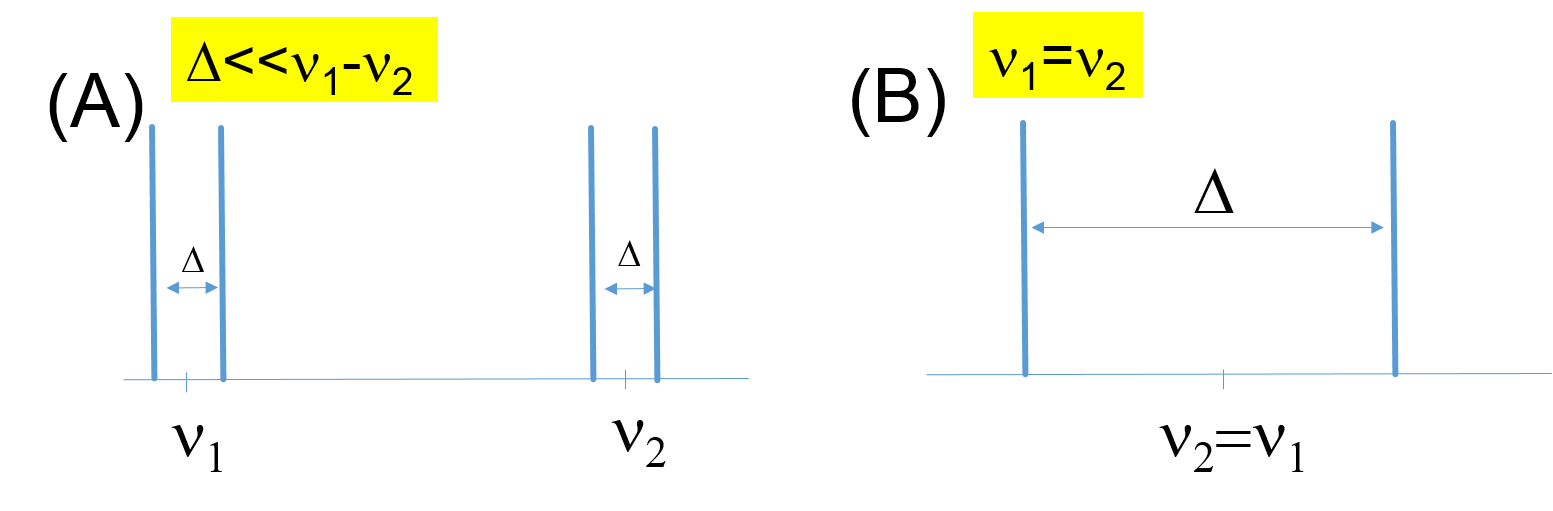
\includegraphics[scale=0.3]{NMRdoublets.png}
    	\caption{Schematic representation of single orientation spectra for (A) $\mid \nu_1 - \nu_2 \mid  \gg \Delta$ and (B) $\nu_1 = \nu_2$.  }
    \end{figure}
\end{frame}
\begin{frame}{\thesection.\thesubsection. \insertsubsection}
	\begin{minipage}[c]{0.3\textwidth}
		\begin{figure} \label{fig:powder_pattern}
			\centering
			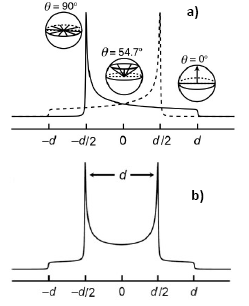
\includegraphics[scale=0.3]{powder_pattern.png}
			\caption{Powder patter dues to a pair of dipolar coupled spins (a) Dotted and continuous lines correspond to different transition. Angles shows related to continous line. (b) Sum of contributions. $d = \dfrac{3 \Delta}{2}$}
		\end{figure}
	\end{minipage}
	\hspace{0.1cm}
	\begin{minipage}[c]{0.65\textwidth}
       In most solids  multiple spins interact via dipolar couplings, but in crystals of CaSO\textsubscript{4}$\cdot$2H\textsubscript{2}O the water molecules are rather isolated from one another approximating an isolated pair. Studying the spectra as a function of crystal orientation help obtain orientational information. \\
       In polycrystalline samples (powders) all values of $\theta$ will be simultaneously present and the spectrum is formed from a weighted superposition of the lines generated by the two transitions for all $\theta$-values. The weighting related to the number of spin-pairs whose inter-nuclear vector takes a particular values of $\theta$. This varies as $\sin \theta$ so that a "powder pattern" in the spectrum takes the form shown in Fig.\ref{fig:powder_pattern}
.       
	\end{minipage}
	

\end{frame}

	
\begin{frame}{\thesection.\thesubsection. \insertsubsection}
		The characteristic spectra shape is called \alert{"powder pattern"}. The two sharp features are called \alert{Pake doublet}.
		\begin{figure}
			\centering
			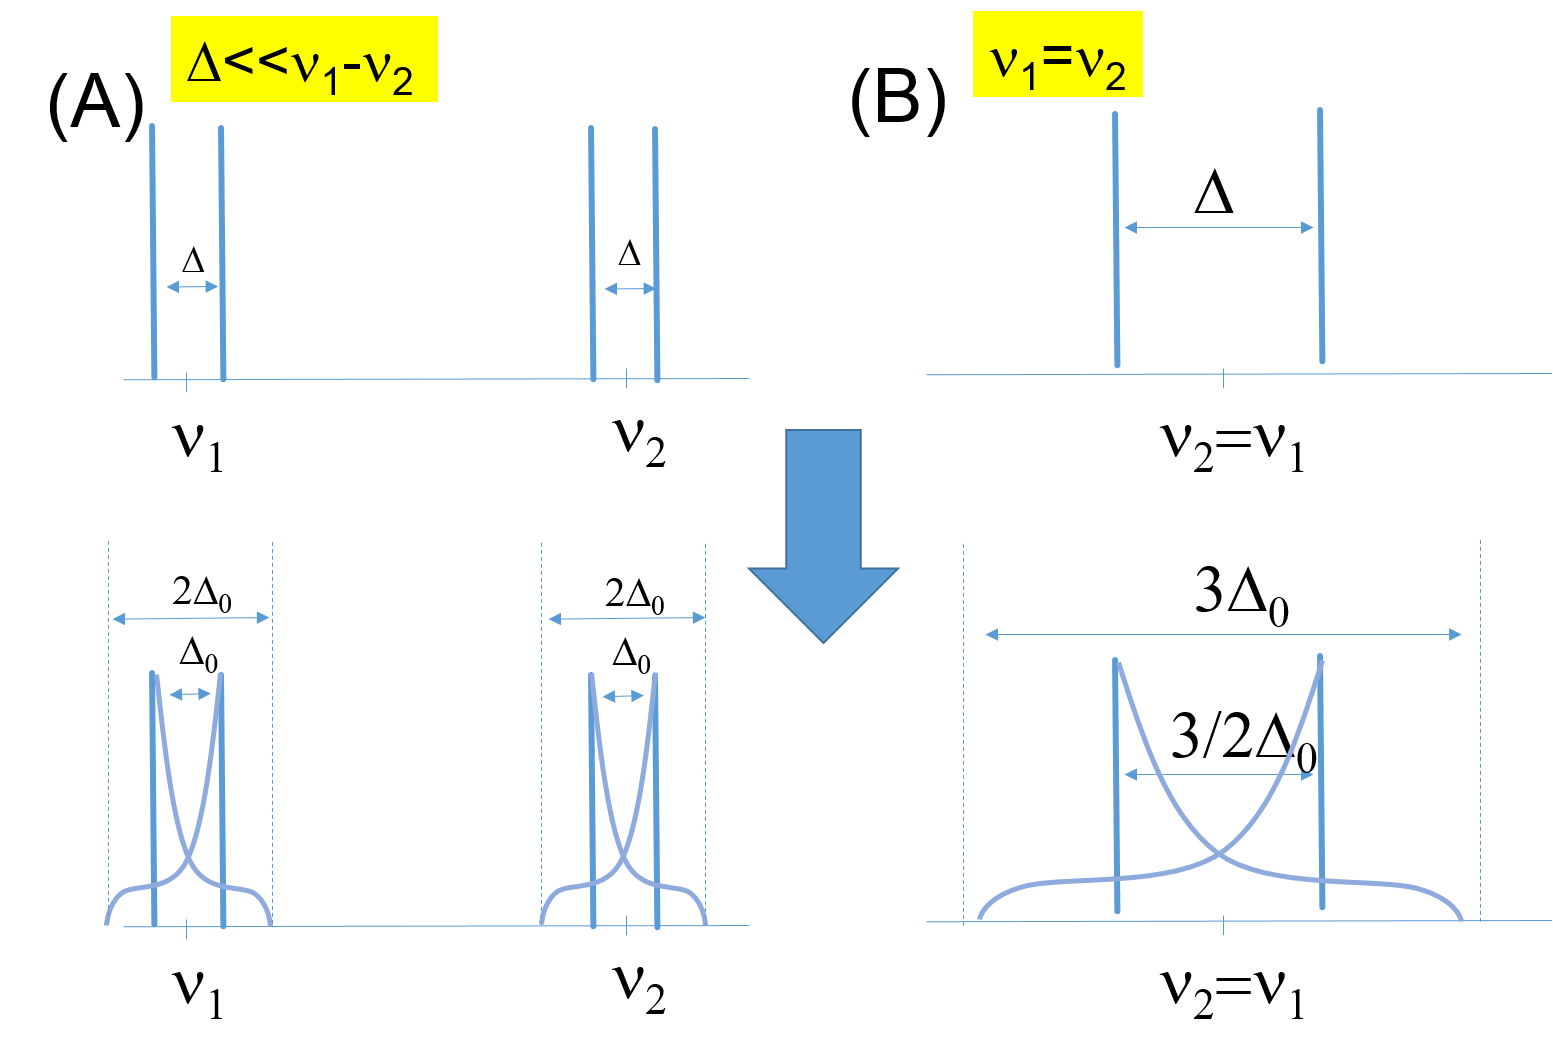
\includegraphics[scale=0.3]{powder_pattern2.png}
				\caption{Schematic representation of polycrystalline spectra for (A) $\mid \nu_1 - \nu_2 \mid  \gg \Delta_0$,  and (B) $\nu_1 = \nu_2$, where $\Delta_0= \dfrac{\mu_0}{8 \pi^2} \dfrac{ \gamma_1 \gamma_2 \hbar}{ r^3}$ }
		\end{figure}
\end{frame}

\subsection{Chemical shift anisotropy.}
\begin{frame}{\thesection.\thesubsection. \insertsubsection}
	Raw NMR spectra from solids often form single broad peaks due to dipolar effects, along with the effects of chemical shift anisotropy, which often makes interpretation of spectra more complicated.
    \begin{figure}
    	\centering
    	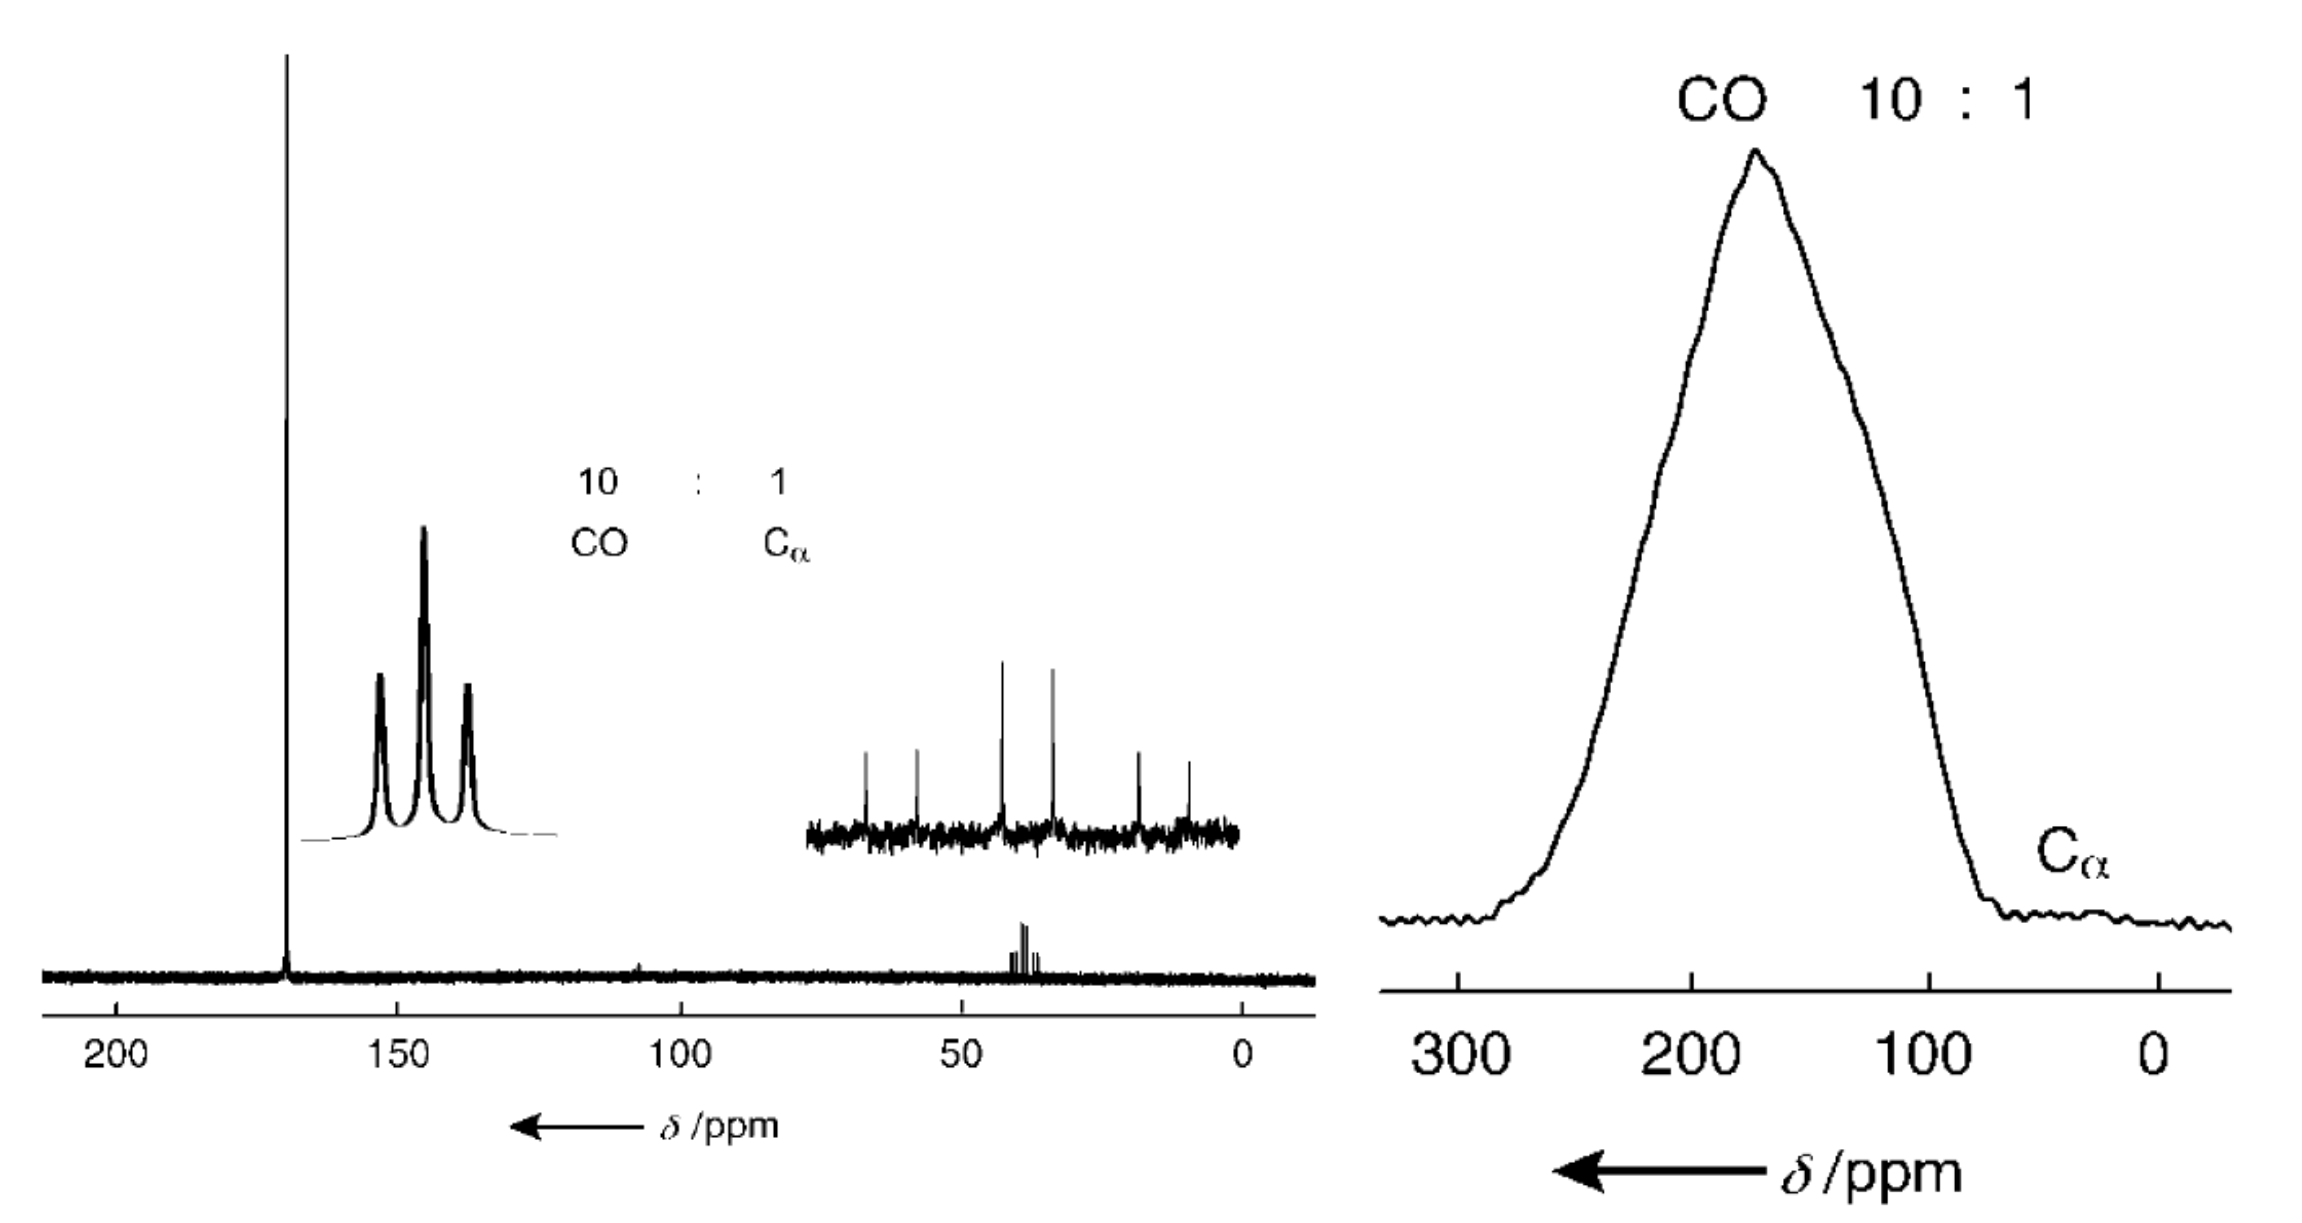
\includegraphics[scale=0.1]{solid-liquid_NMR.png}
    	\caption{\textsuperscript{13}C NMR spectrum of 13C-labelled glycine: (a) 125 MHz solid state; (b) 75 MHz liquid state. From D.D. Laws, H.-M. Bitter, A.Jerschow., Angew. Chem. Int. Ed. 41, 3096 (2002) }
    \end{figure}
\end{frame}

\begin{frame}{\thesection.\thesubsection. \insertsubsection}
	Chemical shift anisotropy results from the dependence of the level of shielding of a nucleus on the orientation of nearby bonds with respect to the magnetic field.
	
	\begin{figure}
		\centering
		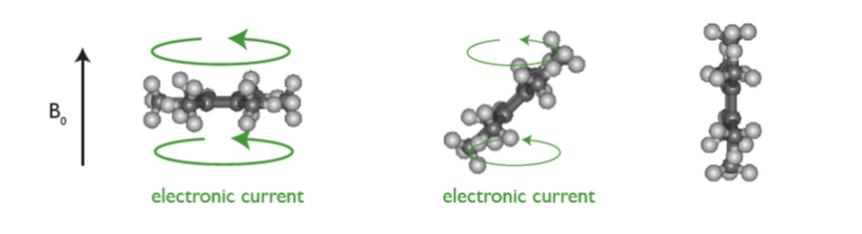
\includegraphics[scale=0.1]{CSA1.png}
		\caption{Dependence of shielding on the molecular orientation with respect to external magnetic field. (\url{www.solidstatenmr.org.uk})}
	\end{figure}	
	
	The effect is characterized by a shielding tensor which relates the induced shielding $\bm{\delta B}$ to the applied field $B_0$ taking into account the orientational dependence.
	
	\begin{equation}
       \begin{bmatrix}
          \delta B_x \\
          \delta B_y \\
          \delta B_z \\
       \end{bmatrix} = -
       \begin{bmatrix}
       \sigma_{xx} & \sigma_{xy} & \sigma_{xz} \\
       \sigma_{yx} & \sigma_{yy} & \sigma_{yz} \\
       \sigma_{zx} & \sigma_{zy} & \sigma_{zz} \\
       \end{bmatrix} 
       \begin{bmatrix}
       0 \\ 
       0 \\
       B_0 \\
       \end{bmatrix}        
	\end{equation}
	
	This introduces a term in the Hamiltonian of the form, $\hat{H}_{CSA} = - \gamma (\bm{\delta B} \cdot \bm{\hat{I}})$.
	
	
\end{frame}


\begin{frame}{\thesection.\thesubsection. \insertsubsection}
    In secular approximation, when the nuclear Zeeman interaction $\gamma B_0 \gg \gamma \sigma_{i,j} B_0$, which is why the secular spin Hamiltonian is truncated to:
    \begin{equation}
       \hat{H_{CSA}} = \gamma \sigma_{zz} B_0
    \end{equation}
    In the laboratory frame in order  $\sigma_{zz}$ component can be found from a full tensor using a product with a unit vector along the direction of $B_0$:
    \begin{equation} \label{eq:sigma_zz}
       \sigma_{zz}^{lab}= 
       \begin{bmatrix}
          0 & 0 & 1
       \end{bmatrix}       
      \begin{bmatrix}
      \sigma_{xx} & \sigma_{xy} & \sigma_{xz} \\
      \sigma_{yx} & \sigma_{yy} & \sigma_{yz} \\
      \sigma_{zx} & \sigma_{zy} & \sigma_{zz} \\
      \end{bmatrix}       
      \begin{bmatrix}
      0 \\
      0 \\
      1 \\
      \end{bmatrix} = \bm{b_0}^{\rm T} \bm{\sigma} \bm{b_0}
    \end{equation}
\end{frame}

\begin{frame}{\thesection.\thesubsection. \insertsubsection}

   In the principle axis system the tensor has the following form:
   \begin{equation}
     \bm{\sigma}=
      \begin{bmatrix}
  	\sigma_{1} & 0 & 0 \\
  	0 & \sigma_{2} & 0 \\
  	0 & 0 & \sigma_{3} \\
  \end{bmatrix}    
   \end{equation}
   The expression in Eq.\ref{eq:sigma_zz} is a true scalar, i.e. it does not depend in which reference frame it is written. We can write it in the principle axis system of the tensor, where the direction of magnetic field is $\bm{b_{PAS}} = \begin{bmatrix} \sin \theta \cos \phi, & \sin \theta \sin \phi,   & \cos \theta \end{bmatrix}  $.
   \begin{align}
      \sigma_zz^{lab} &= \bm{b_0}^{\rm T} \bm{\sigma^{lab}} \bm{b_0} = \bm{b_{PAS}}^{\rm T} \bm{\sigma^{PAS}} \bm{b_{PAS}} = \\
      &= \sigma_1 \sin^2 \theta \cos^2 \phi + \sigma_2 \sin^2 \theta \sin^2 \phi + \sigma_3 \cos^2 \theta 
   \end{align}

\end{frame}   
\begin{frame}{\thesection.\thesubsection. \insertsubsection}
    PAS axis are usually chosen such that  $\sigma_3$ component is the largest. We can use a more convenient notation, by replacing:
    \begin{align}
       \sigma_{iso} &= \dfrac{\sigma_1  + \sigma_2 + \sigma_3}{3}  \text{- isotropic chemical shift} \\
       \Delta &= \sigma_3 - \sigma_{iso} \text{- anisotropy} \\
       \eta &= \dfrac{\sigma_1 - \sigma_2}{\sigma_3} \text{- asymmetry}
    \end{align}
    Using this notation the $\sigma_{zz}^{lab}$ can be found using a compact equation:
    \begin{equation}
       \sigma_{zz}^{lab} = \sigma_{iso} + \dfrac{\Delta}{2}(3 \cos^2 \theta -1 + \eta \sin^2 \theta \cos 2 \phi)
    \end{equation}
\end{frame}

\subsection{Magic angle spinning.}
\begin{frame}{\thesection.\thesubsection. \insertsubsection}
    Magic angle spinning is a technique where the sample is rapidly spun around the axis tilted with respect to $54.5 \deg$ with respect to magnetic field. It allows to removing (almost) all anisotropy arising from the dipolar and CSA interactions. 
    For instance, for dipolar interaction consider two nuclei $A$ and $B$. Place the beginning of coordinates at $A$, $Z$-axis is pointed along the rotation axis and choose $X,Y$-axis such that magnetic field $\bm{B}$ is in $xz$-plane  $\bm{B} = B_0 \begin{bmatrix} 
    \sin \alpha,  &  0, & \cos \alpha
    \end{bmatrix}$.
    
     The radius-vector connecting the two nuclei:
    \begin{equation}
      \bm{r_{AB}} = r_{AB} 
      \begin{bmatrix} 
        \sin \gamma_{AB} \cos \phi_{AB},  &  \sin \gamma_{AB} \phi_{AB}, & \cos \gamma_{AB}
      \end{bmatrix}
    \end{equation}
    Since the sample is spinning, then:
    \begin{equation}
       \phi_{AB} = \phi_{AB}^0 + \Omega t,
    \end{equation}
    where $\phi_{AB}^0$ is some initial phase. 
\end{frame}

\begin{frame}{\thesection.\thesubsection. \insertsubsection}
   We are interested averaging of $(1 - 3 \cos^2 \theta_{AB})$. Since:
   \begin{equation}
      \cos \theta_{AB} = \dfrac{(\bm{r_{AB}}  \bm{B})}{r_{AB} B_0} = \sin \gamma_{AB} \cos \phi_{AB} \sin \alpha + \cos \gamma_{AB} \cos \alpha
   \end{equation}
   then:
   \begin{align}
     1 - 3 \cos^2 \theta &= 1 - 3 \sin^2 \gamma_{AB} \cos^2 \phi_{AB} \sin^2 \alpha -3 \cos^2 \gamma_{AB} \cos^2 \alpha - \\
     &- 6 \sin \gamma_{AB} \cos_{AB} \sin \alpha \cos \gamma_{AB} \cos \alpha
   \end{align}
   For phases linearly varying with time $\overline{\cos \phi_{AB}} = 0 $,  $\overline{\cos^2 \phi_{AB}} = \dfrac{1}{2} $, therefore:
   \begin{equation} \label{eq: MAS}
      \overline{1-3 \cos^2 \theta_{AB}} = -\dfrac{1}{2}(1 - 3 \cos^2 \alpha)(1 - 3 \cos^2 \gamma_{AB})
   \end{equation}

   
\end{frame}

\begin{frame}
	 When $\alpha$ is to the "magic angle" of $\theta_m =54.7 \deg$, $\cos^2 \theta_m = \dfrac{1}{3}$ and the expression in Eq.\ref{eq: MAS} is zero and independet on $\gamma_{AB}$. It means the dipolar interaction is averaged to zero and it does not show up in the spectrum. 
	 So if the spinning is fast enough (i.e. $\Omega \gg \ \dfrac{\gamma_1 \gamma2 \hbar}{r^3} \text{ or } \gamma \sigma_{max} B_0$  )instead of wide lines due to CSA or dipolar only sharp lines (liquid-state like) spectrum arises. 
\end{frame}

\subsection{Quadrupolar interaction.}
\begin{frame}
	All nuclei with a spin greated that $\dfrac{1}{2}$ have an electric quadrupole moment in a ddition to the magnetic dipole moment, possessed by spin-$\dfrac{1}{2}$ nuclei. Electric quadrupoles interact with electric field gradients. 
	In atoms and molecules the electrons and nuclei create electric fields (and electric field gradients) at the location of a nucleus. Effectively, one can say that electric fields of a molecule tend to reorient a nucleus in a certain way.  Quadrupolar moment is a tensor and is proportional to a tensor combined of spin components (Wigner-Eckart theorem). We will not derive the equation for such coupling, but go straight to the result. The quadrupolar coupling Hamiltonian is:
	\begin{equation}
	   \hat{H_Q} = \dfrac{eQ}{6I(2I-1)\hbar} \sum_{i,j=x,y,z} \hat{I}_i e q_{ij}  \hat{I}_j, 
	\end{equation}
	where $eQ$ is a quadrupole moment, a constant depends only on a nuclear species, $e q_{ij}$ are the components of electric field gradient tensor. 
\end{frame}
\begin{frame}
	
	The quadrupolar interaction tensor is traceless, i.e. has only two independent components. If its principal components are defined as $q_{xx}^{PAS}, q_{yy}^{PAS}, q_{zz}^{PAS}$, then two parameters describing the tensor can be introduced:
	\begin{align}
	   \chi &= \dfrac{e^2 q_{zz}^{PAS} Q}{\hbar}  \text{   -quadrupole coupling constant} \\
	   \eta_Q &= \dfrac{q_{xx}^{PAS} - q_{yy}^{PAS}}{q_{zz}^{PAS}} \text{  -asymmetry parameter}
	\end{align}
	
	In the PAS the hamiltonian has a form:
	\begin{equation}
		\hat{H}_Q = \dfrac{\chi }{4 I (2I-1)}\Big(3 \hat{I}_z^2 - I(I+1) ) + \eta_Q(\hat{I}_x^2 -\hat{I}_x^2)  \Big)
	\end{equation}

\end{frame}	
\begin{frame}


	In case of axial symmetry,$\eta_Q = 0$, the Hamiltonian of a quadrupolar nucleus in the magnetic field:
	\begin{equation}
	   \hat{H} = - \nu_0 \hat{I}_z + \dfrac{\chi}{8} (3 \cos^2 \theta - 1) \dfrac{3 \hat{I}_z^2  -I(I+1) }{I(2I-1)},
	\end{equation}
	where $\theta$ is the direction of the magnetic field in the PAS of quadrupolar tensor. Since the selection rule is $\Delta m_I = \pm1$ the transition frequencies are:
	\begin{equation}
	  \nu = \nu_0 -\dfrac{3}{8} \chi \dfrac{2 m_I -1}{I(2I -1)}(3 \cos^2 \theta - 1)
	\end{equation}
	 
\end{frame}
%%%%% END OF RESONANT ABSORPTION



%\begin{frame}
%
%	These equations describe a precession of a vector $\bm{M}$ around the direction of the external magnetic field $\bm{B}$ with the frequency $\omega_0$ as shown schematically in Fig.\ref{fig:precession}A. Such motion is called  "Larmor precession" and $\omega_0 = \gamma B_0$ is called "Larmor frequency".
%	
%	Of course, this primitive classical picture serves only as an illustration to the actual behaviour of magnetic moments placed into a magnetic field. However, a more rigorous description using quantum mechanics for an ensemble of magnetic moments provides a similar answer. Larmor precession of an overall magnetic moment is a real effect, and as we will see later, it is essential for acquiring of magnetic resonance spectra.
%	
%
%	
%	Now we'll briefly sketch the basic quantum mechanical description of a magnetic moment in a magnetic field.  The angular momentum operator $\bm{\hat{L}}$ (which could be an orbital or spin angular momentum) is proportional to the magnetic moment operator as:
%	\begin{equation} \label{eq:3}
%	\bm{\hat{\mu}} = \gamma \hbar \bm{\hat{L}},
%	\end{equation}
%	The Hamiltonian of a system can be written by analogy with expression \ref{eq:2} as:
%	\begin{equation} \label{eq:2level}
%	\hat{H} = -\bm{\hat{\mu}} \bm{B} = -\gamma \hbar \hat{I}_{z} B_0 = -\omega_0 \hat{I}_{z},
%	\end{equation}
%	
%	The level diagram in Fig.\ref{fig:precession}B shows schematically the splitting of $\gamma \hbar B_0 $ between energy levels  as a function of the applied magnetic field for a system with only a spin-$\frac{1}{2}$ angular momentum. In this case, the eigenfunctions corresponding to the two energy levels are just the two projections of a spin onto the $z$-axis: $m_z=+\frac{1}{2}$ is $\vert \alpha \rangle$ and $m_z=-\frac{1}{2}$ is $\vert \beta \rangle$.
%	
%	
%\end{frame}

\end{document}